% should be sigplan instead of acmsmall?
\documentclass[acmsmall]{acmart}
%%
%% \BibTeX command to typeset BibTeX logo in the docs
\AtBeginDocument{%
  \providecommand\BibTeX{{%
    Bib\TeX}}}

\usepackage{tikz}
\usepackage{mathpartir}
%\usepackage[colorlinks=true, linkcolor=blue]{hyperref}
\usepackage[capitalise]{cleveref}
\usepackage{xcolor} 
\usepackage{hyperref}
\usepackage{bussproofs}
% this doesn't seem to be working...
\hypersetup{
    colorlinks=true,
    linkcolor=blue,
    urlcolor=cyan,
    }

%\crefname{figure}{figure}{figures}
%\Crefname{figure}{Figure}{Figures}



%% Commands
\newcommand{\rec}{\mathsf{rec}}
\newcommand{\VType}{\mathbf{VType}}
\newcommand{\CType}{\mathbf{CType}}
\newcommand{\Prop}{\mathbf{Prop}}

\newcommand{\isVType}{\textrm{ VType}}
\newcommand{\isCType}{\textrm{ CType}}
\newcommand{\isProp}{\textrm{ Prop}}
\newcommand{\isCtx}{\textrm{ Ctx}}

\newcommand{\ctxjdg}[1]{#1 \isCtx}
\newcommand{\vtypejdg}[2]{#1 \vdash #2 \isVType}
\newcommand{\ctypejdg}[2]{#1 \vdash #2 \isCType}
\newcommand{\vtrmjdg}[3]{#1 \vdash #2 : #3}
\newcommand{\ctrmjdg}[3]{#1 \vdash #2 : #3}

\newcommand{\den}[1]{\llbracket #1\rrbracket}
\newcommand{\denLctx}[1]{\den{#1}^L_{ctx}}
\newcommand{\denLty}[1]{\den{#1}^L_{ty}}
\newcommand{\denLtm}[1]{\den{#1}^L_{tm}}

\newcommand{\obliv}[2]{\mathcal{O}_{#1}({#2})}
\newcommand{\wrap}[2]{\mathcal{W}_{#1}({#2})}


\newcommand{\bool}{\mathbb{B}}
\newcommand{\true}{\mathtt{true}}
\newcommand{\false}{\mathtt{false}}
\newcommand{\nat}{\mathbb{N}}

\newcommand{\eric}[1]{\textcolor{red}{ <eric-#1> }}
\newcommand{\source}{$\mathbf{F}_{\mu,\Omega}^{\forall\to}\;$}
\newcommand{\pl}{$\mathbf{PL}$}
\newcommand{\fpl}{$\mathbf{FPL}$}



%% Rights management information.  This information is sent to you
%% when you complete the rights form.  These commands have SAMPLE
%% values in them; it is your responsibility as an author to replace
%% the commands and values with those provided to you when you
%% complete the rights form.
\setcopyright{acmlicensed}
\copyrightyear{2018}
\acmYear{2018}
\acmDOI{XXXXXXX.XXXXXXX}
%% These commands are for a PROCEEDINGS abstract or paper.
\acmConference[Conference acronym 'XX]{Make sure to enter the correct
  conference title from your rights confirmation email}{June 03--05,
  2018}{Woodstock, NY}
%%
%%  Uncomment \acmBooktitle if the title of the proceedings is different
%%  from ``Proceedings of ...''!
%%
%%\acmBooktitle{Woodstock '18: ACM Symposium on Neural Gaze Detection,
%%  June 03--05, 2018, Woodstock, NY}
\acmISBN{978-1-4503-XXXX-X/2018/06}


%% Submission ID.
%% Use this when submitting an article to a sponsored event. You'll
%% receive a unique submission ID from the organizers
%% of the event, and this ID should be used as the parameter to this command.
%%\acmSubmissionID{123-A56-BU3}


\begin{document}

%%
%% The "title" command has an optional parameter,
%% allowing the author to define a "short title" to be used in page headers.
\title{Fresh Parametricity}


\author{Eric Bond}
\email{bonderic@umich.edu}
\affiliation{%
  \institution{University of Michigan}
  \city{Ann Arbor}
  \country{USA}
}

\author{Max New}
\affiliation{%
  \institution{University of Michigan}
  \city{Ann Arbor}
  \country{USA}
}

%%\renewcommand{\shortauthors}{Trovato et al.}


\begin{abstract}
Recent works combining parametric polymorphism with language features relying on intensional type analysis have lead to non-standard definitions of parametricity. The relative strength of traditional vs these type-world notions of parametricity remains an open question. We shed some light on this issue by framing this question as a matter of translation between logics. To this end, we define two logics for proving theorems about parametricity, one traditional and one based on fresh parametricity, and we demonstrate a translation which preserves logical equivalence. 

\end{abstract}

%%
%% The code below is generated by the tool at http://dl.acm.org/ccs.cfm.
%% Please copy and paste the code instead of the example below.
%%
\begin{CCSXML}
<ccs2012>
 <concept>
  <concept_id>00000000.0000000.0000000</concept_id>
  <concept_desc>Do Not Use This Code, Generate the Correct Terms for Your Paper</concept_desc>
  <concept_significance>500</concept_significance>
 </concept>
 <concept>
  <concept_id>00000000.00000000.00000000</concept_id>
  <concept_desc>Do Not Use This Code, Generate the Correct Terms for Your Paper</concept_desc>
  <concept_significance>300</concept_significance>
 </concept>
 <concept>
  <concept_id>00000000.00000000.00000000</concept_id>
  <concept_desc>Do Not Use This Code, Generate the Correct Terms for Your Paper</concept_desc>
  <concept_significance>100</concept_significance>
 </concept>
 <concept>
  <concept_id>00000000.00000000.00000000</concept_id>
  <concept_desc>Do Not Use This Code, Generate the Correct Terms for Your Paper</concept_desc>
  <concept_significance>100</concept_significance>
 </concept>
</ccs2012>
\end{CCSXML}

\ccsdesc[500]{Do Not Use This Code~Generate the Correct Terms for Your Paper}
\ccsdesc[300]{Do Not Use This Code~Generate the Correct Terms for Your Paper}
\ccsdesc{Do Not Use This Code~Generate the Correct Terms for Your Paper}
\ccsdesc[100]{Do Not Use This Code~Generate the Correct Terms for Your Paper}

%% Keywords. The author(s) should pick words that accurately describe
%% the work being presented. Separate the keywords with commas.
\keywords{Do, Not, Us, This, Code, Put, the, Correct, Terms, for,
  Your, Paper}


\received{20 February 2007}
\received[revised]{12 March 2009}
\received[accepted]{5 June 2009}


\maketitle

\section{Introduction}
\eric{rephrase "type instantiations"}
\eric{rephrase "variant of System F"}
\eric{fresh param instead of non-standard?}
\eric{consistency in inclusion/exclusion of stoup}
\subsection{Parametricity}
\eric{this is word vomit. decide how you want to introduce parametrictiy, then work on flow}
Parametricity states \eric{wording}that any term of a universal or existential type must behave uniformly for any possible type instantiation.
Existential types can be used to encode abstract data types like Queues or Graphs. 
If we know our language enjoys parametric polymorphism, then we have a guarantee that any two instance of a Queue, as encoded by an existential type, are observationally equivalent.
Meaning, we can swap implementations of the Queue data type without changing the correctness of the overall program. (ignoring resource constraints, time/space)
Universal types in a parametrically polymorphic language allow for a sound implementation of church encoded data. 
Theorems for free
	\eric{
	Address this first, then provide examples?}

\subsection{Parametricity vs Intensional Type Analysis}
\eric{Dyn or ?}
While parametricity is a desirable property, it is hard to maintain with certain language features that use \textit{intensional type analysis} \cite{IntTypeAnalysis}. By Intensional type analysis, we mean the ability to inspect the run time representaiton of a type and dispatch based on the result. \eric{wording}An example of this behavior is the casting rules in a gradual typed language\cite{GradParam}.


\subsubsection{Gradual Typing}
Gradual typing allows programmers gradually migrate from \eric{dynamically/untyped} code to typed code by including a type $Dyn$ representing a dynamically checked term. 
The interface between dynamically typed code and statically typed code is handled by casting.
A value of any type $A$ can be up cast $\uparrow_A^?$ to the dynamic type.
Downcasting $\downarrow_A^?$from the dynamic type can introduce errors if the value stored in Dyn is not of the requested type.
Naively adding Dyn, up casting, and down casting to a parametrically polymorphic language breaks parametricity. 
Consider a polymorphic gradually typed language which can error.
$$t : \forall X. X \rightarrow \mathbb{B}:= (\Lambda X. \lambda (x : X). \downarrow_\mathbb{B}^?\uparrow_X^?(x))$$

\eric{$\mathbb{B}$ and Bool used here}
If we assume that $t$ behaved uniformly for all possible type instantiations, then $t$ should either error
or return a boolean that is not dependent on the argument of type $X$.
But this is not the case
when instantiated at type Bool, $t$ will return the given boolean value
$t[\mathbb{B}](b : \mathbb{B}) \leadsto^* b$ for any other type $A$ it will error
$t[A](x:A)\leadsto^* \Omega$
Therefore $t$ does not behave uniformly for all types. 
The issue here is that casting inspects the type tag used in the values stored in dyn, a case of intensional type analysis.

\subsection{Preserving Parametricity}
% many attempts to combine gradual typing and parametric polymorphism
% it has been demonstrated 

% Not just gradual typing.. intensional type analysis
The difficulties of combining parametric polymorphism and language features relying on type analysis are well known\cite{NonParam}\cite{GradParam}\cite{ToroGradParam}\cite{ForFreeForFree}.
Solutions that preserve parametricity usually involve a form of \textit{dynamic sealing} or generation of \textit{fresh type tags}. Reason being, the ability to inspect a type and dispatch based on the result is in direct conflict with the information hiding principle provided in a language with parametric polymorphism. By hiding information about the runtime representation of a type, we can restore the property that polymorphic types behave uniformly across all type instantiations.

While such techniques have demonstrated they can preserve the expected information hiding properties, they do so using a \textit{non-standard} formulation of parametricity. Specifically, the approach used by Niels\cite{NonParam} and New\cite{GradParam} invoke a \textit{Type-World} logical relation where the freshly allocated type variables/tags, $\alpha$, are associated with concrete types, $(A,A')$, and a relation, $R : Rel[A,A']$, on those types. This mapping, $\alpha \mapsto (A,A',R)$, of dynamically allocated type variable to concrete types and a relation are threaded through the logical relation via a Kripke world. A question remains, what is the relative strength of this non-standard formulation of parametricity compared to traditional definitions? In particular, does the \textit{type-world} formulation allows us to prove the \textit{free-theorems} and \textit{data-abstraction} properties we would should expect?\eric{introduce vocab? non-starndard param as type world param?}

\subsection{Failure of Full Abstraction}
This was partially answered in the affirmative by Nies et al\cite{NonParam}. The argument proceeds by introducing two languages: An effectful variant of CBV System F with a standard notion of parametricity, and System G, an extension of the former language with type casts and fresh type name allocation supporting a \textit{non-standard}, type world, formulation of parametricity.
To compare the languages, they provide a type preserving embedding, $\den{\_}$, from System F to System G. 
  $$\vdash_F V : A \implies \vdash_G \den{V} : \den{A}$$

The embedding, $\den{\vdash_F V:A} = \mathcal{W}_{A} \circ \den{\vdash_F V:A}^L$, is decomposed into a lifting, $\den{\_}^L$, and a type directed wrapping function $\mathcal{W}_A$. The lifting preserves syntactic equality of terms and types, so $V \equiv \den{V}^L$ and $A \equiv \den{A}^L$. The wrapping function is a deep $\eta$ expansion which strategically inserts fresh type allocation in the elimination forms of the universal and existential types. The purpose of the wrapping is to ensure that lifted polymorphic terms of System F are simultaneously safe from non-parametric uses and forced to behave parametrically in the presence of System G's type cast operation. More details can be found in \cref{sec:Wrap}. 

\begin{conjecture}
  \textbf{False}: Full Abstraction of $\den{\_}$
  $$\forall V_1,V_2. V_1\cong_F V_2 \iff \den{V_1} \cong_G \den{V_2}$$
\end{conjecture}

To demonstrate the relative strengths of the different notions of parametricity, they conjecture that the embeddings is \textit{fully-abstract}, preserving and reflecting all contextual equivalences. However, this conjecture was later disproven\cite{ParamVSUniv} \cite{TwoParamVSThreeUniv}. In particular, it was shown that contextual equivalence is not preserved by the translation. Specifically, the type $Univ := \exists Y.\forall X. (X\rightarrow Y)\times (Y \rightarrow X)$ must be \textit{degenerate} in effectful System F, but there are non-degenerate inhabitants of this type in System G. \eric{provide explicit counter?}

\subsection{Our Result}
\eric{rename section, more connective tissue}
\eric{TODO: more precision is needed here. Equivalence vs preservation of equivalence vs logical full abstraction which requires Reflection!}
Our aim is to demonstrate that, while the transformation does not preserve contextual equivalence, it preserves a weaker notion we call \textit{Logical Equivalence}. By Logical Equivalence, we mean to say that any results proven in a \textit{Parametricity Logic}\cite{APL}\cite{LAPL}\cite{PE} for effectful System F can be transfered to a parametricity logic backed by the non-standard, type-world, notion of parametricity. By limiting our reasoning principles to a well-defined parametricity logic, we rule out metatheoretical reasoning which was used in prior work\cite{TwoParamVSThreeUniv} to demonstrate that the type $Univ$ is degenerate. We demonstrate that the lack of metatheoretical reasoning principles does not preclude our logic from proving useful properties about data abstraction and representation independence. \eric{hrm.. but we don't include existentials here..}

%y constructing two parametricity logics. One for a language without fresh type generation, another for a language with fresh type generation. We then show that any two provably equal terms of the first logic are provable equal, under translation, in the second logic.
\begin{theorem}
  Preservation of Logical Equivalence (simplified):
  $$\Gamma \vdash_{PL} M = N \implies \den{\Gamma} \vdash_{FPL} \den{M} = \den{N}$$
\end{theorem}



\subsection{Overview}

\eric{bullet format or paragraph?}
 To demonstrate the preservation of logical equivalence we first define \source, an effectful CBV variant of System F in \cref{sec:SourceLang} for which we want our theorem to apply. We then define two logics: \textbf{Parametricity Logic}(\pl) and \textbf{Fresh Parametricity Logic}(\fpl). The \textit{term languages} of these logics, defined in \cref{sec:ObjLang}, are effectful, CBPV \cite{CBPV} variants of System F. Embeddings of \source into \pl and \fpl are covered in \eric{cref}. The embeddings largely follow the usual\cite{CBPV} CBV to CBPV translation, with a few exceptions, notably the parametricity preserving wrapping in \cref{sec:Wrap}. In \cref{sec:Logics}, we will introduce our parametricity logics\eric{cref} and the translation \eric{cref} between the logics.
 \eric{compositionality issues.. oblivious predicate..adequacy..example proof in Logic..discussion/relatedwork.. order TBD here.. come back to this}







\begin{comment}
\subsubsection{Gradual Typing with Fresh Quantification}

To illustrate this, we will consider a polymorphic Call-by-push-value \eric{cite} calculus with an extensible sum type denoted $OSum$ which we use to represent the dynamic type Dyn. In order to inject a value, $V:A$, into $OSum$, we need a $Case$ symbol associated with the type $A$. Case symbols are representative of the runtime type tags of the dynamic type and can be dynamically allocated by the expression $new_A : F(Case\;A)$. The introduction from of the extensible sum type, $inj_\sigma\;V : OSum$ uses a case symbol $\sigma : Case\;A$ to store a value $V:A$. The elimination form, $rec_{OSum}\;(inj_\sigma\;V),\sigma'\;\{x.\;M\;|\;N\}$, compares the case symbol $\sigma$ used to inject the value into $OSum$ to a given case symbol $\sigma'$. When the case symbols match, the value stored in $OSum$ is bound to $x$ in the continuation $M$. Otherwise, we proceed with the default case $N$. Assuming a preallocated set of case symbols $\sigma_\mathbb{B} : Case\;\mathbb{B},\sigma_\times : Case\;(OSum \times OSum),\sigma_\to : Case\;(OSum \to OSum),...$, we can encode the example above as:
$$t : \forall X.Case\;X \to X \to F\mathbb{B} := \Lambda X. \lambda \sigma_X.\lambda x.rec_{OSum}\;(inj_{\sigma_X}x),\sigma_\mathbb{B}\;\{x.\;ret\;x\;|\;\Omega\}$$
\\
\\
% preserve parametricity reasoning?
\end{comment}




\section{Languages}\label{sec:Languages}
\begin{itemize}
  \item section overview.
  \item why have a source language
  \item why CBPV
\end{itemize}
\eric{redo}
In this section we introduce \source, an effectful variant of CBV System F, two versions of an effectful CBPV variant of System F with and without fresh case allocation. \eric{more exposition}

\subsection{Source Language}\label{sec:SourceLang}
\begin{itemize}
  \item why polymorphic multi-arg function type?
  \item why general recursion and error? (OSum can encode these)
\end{itemize}
\source is mostly a standard polymorphic, CBV language with general recursion and the ability to raise errors. One major difference being that we replace the universal quantification and function type with a polymorphic, multi-argument function type, similar to that of $\lambda^K$\cite{SysFtoTAL}. Notably, this type does not support partial application; a trade-off we accept for finer control over equational reasoning, as discussed in \cref{sec:SourceToPL}.

\begin{figure}[H]
  \begin{mathpar}
    \scriptsize
    \inferrule{ }{\Gamma,X \vdash X \; Type}
    \and
    \inferrule{ }{\Gamma \vdash \mathbb{B} \; Type}
    \and
    \inferrule{ }{\Gamma \vdash \mathbb{N} \; Type}
    \and
    \inferrule{\Gamma \vdash A \; Type \\ \Gamma \vdash A' \; Type}
              {\Gamma \vdash A \times A' \; Type}
    %\and
    %\inferrule{\Gamma,X \vdash A \; Type}
     %         {\Gamma \vdash \exists X.A}
    \and
    \inferrule{\Gamma,\overrightarrow{X}_n \vdash A_i \; Type \;\;\forall i \in \{m\} \\
               \Gamma,\overrightarrow{X}_n \vdash A \; Type}
              {\Gamma \vdash \forall[\overrightarrow{X}_n].(\overrightarrow{A}_m)\rightarrow A \; Type}
  \end{mathpar}
  \caption{Type Formers: \source}
  \label{fig:value-type-formers}
\end{figure}


\begin{figure}[H]
  \begin{mathpar}
    \scriptsize
    \inferrule{ }{\Gamma ,x : A \vdash x : A}

    % Bool
    \and
    \inferrule{ }{\Gamma \vdash true : \mathbb{B}}
    \and
    \inferrule{ }{\Gamma \vdash false : \mathbb{B}}
    \and
    \inferrule{\Gamma \vdash b : \mathbb{B} \\ \Gamma \vdash M : A \\ \Gamma \vdash N : A}
              {\Gamma \vdash rec_{\mathbb{B}} \;b \; \{M\;|\;N\} : A}

    % Nat
    \and
    \inferrule{ }{\Gamma \vdash z : \mathbb{N}}
    \and
    \inferrule{\Gamma \vdash n : \mathbb{N}}
              {\Gamma \vdash s\;n : \mathbb{N}}
    \and
    \inferrule{\Gamma \vdash n : \mathbb{N} \\ \Gamma \vdash M : A \\ \Gamma,x : \mathbb{N} \vdash N : A}
              {\Gamma \vdash rec_{\mathbb{N}} \;n \; \{M\;|\; x.\;N\} : A}

    % Jumbo Function
    \and
    \inferrule{\Gamma,\overrightarrow{X}_n\vdash A_i \;Type\;\; \forall i\in \{m\} \\
              \Gamma,\overrightarrow{X}_n\vdash A' \;Type \\
              \Gamma,\overrightarrow{X}_n,x_1 : A_1,\cdots,x_m : A_m \vdash M : A'}
              {\Gamma \vdash \Lambda[\overrightarrow{X}_n](x_1 : A_1,\cdots,x_m:A_m).M : \forall[\overrightarrow{X}_n].(\overrightarrow{A}_m)\rightarrow A'}

    \and
    \inferrule{\Gamma \vdash A_i\;Type \;\;\forall i\in \{n\} \\
              \Gamma \vdash M : \forall[\overrightarrow{X}_n].(\overrightarrow{A}_m) \rightarrow A' \\
              \Gamma \vdash N_i : B_i[\overrightarrow{A}/\overrightarrow{X}] \; \forall i \in \{m\}}
              {\Gamma\vdash M[\overrightarrow{A}_n](N_1 : B_1,\cdots N_m : B_m) : A'}

    % Exists
    %\and
    %\inferrule{\Gamma \vdash V : T[A/X]}
    %          {\Gamma \vdash pack\langle A,V \rangle : \exists X. T}
    %\and
    %\inferrule{\Gamma  \vdash W : \exists X.T \\ \Gamma,A,V:T[A/X] \vdash M : A'}
    %          {\Gamma \vdash unpack\langle A, V\rangle = W; M : A'}

    % Product
    \and
    \inferrule{\Gamma \vdash M : A \\ \Gamma \vdash N : A}
              {\Gamma \vdash (M,N) : A \times A}
    \and
    \inferrule{\Gamma \vdash M : A\times A' \\ \Gamma,x:A,y:A' \vdash N : A}
              {\Gamma \vdash rec_\times \; M \;\{x,y.\; N\} : A''}

    % Error
    \and
    \inferrule{ }{\Gamma \vdash \Omega_A : A}

    % Fixpoint
    \and
    \inferrule{\Gamma , x : A \vdash V : A'}
              {\Gamma \vdash \mu x . V : A'}
\end{mathpar}
\caption{Typing Rules:\source}
\label{fig:value-type-formers}
\end{figure}





\subsection{\pl \; \& \fpl \;Term Languages}\label{sec:ObjLang}
\begin{itemize}
  \item remark: mixed term/type context
  %\item explain: Why $\forall \underline{X}.\underline{B}$ and no $F$? Justify church encoding here or later? Provide definition of church encoded $ret$ and $bind$? will likely use later.. 
  %\item describe: $OSum,Case\;A$
  \item remark: how $new$ is presented as an effect? (its church encoding)
  %\item remark: inclusion of Observation type (b/c church encoded F)
  \item remark: exclusion of $\underline{B} \multimap \underline{B}' $ 
  type 

  %\item \eric{TODO: remove exists}
  \item \eric{TODO: rephrase "object language"}
  %\item \eric{TODO: include complex values (disclose motivation? the wrapping definition)}
  %\item \eric{operational behavior..? perhaps not if we don't discuss models}
  %\item \eric{equational theory here? or in the Logic section?} \href{https://publish.obsidian.md/2025/PhD/Shared/Parametricity+Logic/Result/Object+Language#Equational+Theory}{equations link}
\end{itemize}

Here we introduce the term languages for \pl \;and \fpl. These are based on a polymorphic CBPV calculus with an error effect and general recursion. We include an observation type, $Obs$, with no elimination form. Two notable difference are the inclusion of an extensible sum type $OSum$ and absence of the computation type $FA$.

\begin{figure}[H]
  \centering
  \scriptsize
  
  % --------- Contexts ---------
  \textbf{Contexts}
  \begin{mathpar}
  \inferrule{ }{ \ctxjdg{\cdot} }
  
  \inferrule{\ctxjdg{\Gamma} \\ \vtypejdg{\Gamma}{A}}
            { \ctxjdg{\Gamma,A} }
  
  \inferrule{\ctxjdg{\Gamma} \\ \ctypejdg{\Gamma}{\underline{B}}}
            { \ctxjdg{\Gamma,\underline{B}} }
  
  \inferrule{\ctxjdg{\Gamma} \\ \vtypejdg{\Gamma}{A}}
            { \ctxjdg{\Gamma,x:A} }
  \end{mathpar}
  
  
  % --------- Value Type Formers ---------
  \textbf{Value Types}
  \begin{mathpar}
  \inferrule{ }{ \vtypejdg{\Gamma}{0} }
  
  \inferrule{ }{ \vtypejdg{\Gamma}{\mathbb{B}} }
  
  \inferrule{ }{ \vtypejdg{\Gamma}{\mathbb{N}} }
  
  \inferrule{X \in \Gamma}
            { \vtypejdg{\Gamma}{X} }
  
  \inferrule{\ctypejdg{\Gamma}{\underline{B}}}
            { \vtypejdg{\Gamma}{U\underline{B}} }
  
  \inferrule{\vtypejdg{\Gamma}{A} \\ \vtypejdg{\Gamma}{A'}}
            { \vtypejdg{\Gamma}{A \times A'} }
  
  \colorbox{lightgray}{${\inferrule{ }{ \vtypejdg{\Gamma}{OSum} }}$}
  
  \colorbox{lightgray}{$\inferrule{\vtypejdg{\Gamma}{A}}
            { \vtypejdg{\Gamma}{Case \; A} }$}
  \end{mathpar}
  
  \vspace{.5em}
  
  % --------- Computation Type Formers ---------
  \textbf{Computation Types}
  \begin{mathpar}
  \inferrule{\underline{X} \in \Gamma}
            { \ctypejdg{\Gamma}{\underline{X}} }
  
  \inferrule{ }{ \ctypejdg{\Gamma}{Obs} }
  
  \inferrule{\vtypejdg{\Gamma}{A} \\ \ctypejdg{\Gamma}{\underline{B}}}
            { \ctypejdg{\Gamma}{A \to \underline{B}} }
  
  \inferrule{ \ctypejdg{\Gamma, X}{\underline{B}} }
            { \ctypejdg{\Gamma}{\forall X . \underline{B}} }
  
  \inferrule{ \ctypejdg{\Gamma, \underline{X}}{\underline{B}} }
            { \ctypejdg{\Gamma}{\forall \underline{X} . \underline{B}} }
  \end{mathpar}
  
  \caption{Contexts, Value Types, and Computation Types: \pl \; \& \colorbox{lightgray}{\fpl}}
  \label{fig:combined-object-language-clean}
  \end{figure}


\subsubsection{Extensible Sum Type}\label{sec:OSum}
In order to study parametricity in the presence of type analysis, we include an extensible sum type, $OSum$, along with the type $Case\;A$ as a proxy for the dynamic type and first class representaiton of type tags. Thus, instead of including a type case operation ala System G\cite{NonParam}, we adopt a form of type analysis used in gradual typing where type tags of the dynamic type can be inspected. Following prior work on combining gradual typing and parametricity \cite{GradParam}, we reinterpret the universal type $\forall X. \underline{B}$ as the \textit{fresh universal type} $\forall X. Case\:X \rightarrow \underline{B}$ in our type translation(\cref{fig:TypeTranslationPLFPL}) between \pl\; and \fpl.


$$
\sigma \leftarrow new_{\mathbb{B}}; ret\; inj_\sigma (true) : F(OSum)
$$
In order to inject a value $V : A$ into $OSum$, we must first have a case symbol $\sigma : Case\;A$ for type $A$, which can be dynamically allocated using $new_A$. 
To eliminate $V : OSum$, we compare a given $\sigma : Case\;A$ to the case symbol which was used to construct the value $V$. When the cases match, we have a continuation, $x.\;M$, which receives the value which was stored in the sum. Otherwise, we proceed to a default computation $N$. 


\subsubsection{Church Encoded $F$}\label{sec:ChurchEncF}
Following prior work on parametricity logics with effects\cite{PE}, our calculi do not contain a first class computation type $FA$. Instead, $FA$ is church encoded so that its relational interpretation is inherited from its component types. Unlike typical church encoded data, $FA$ uses universal quantification over computation types rather than value types. Relational interpretation of types can be found in \cref{todo}
\begin{figure}[H]
  \centering
  \scriptsize
  \begin{align*}
    &FA := \forall \underline{X}.U(A \to \underline{X}) \to \underline{X}\\
    &ret\;V : F A := \Lambda \underline{X}.\lambda k:U(A \to \underline{X}). (force\; k)V\\
    &(x \leftarrow M; N) : \underline{B}:= M[\underline{B}](thunk(\lambda x : A.N))
  \end{align*}
  \caption{Church Encoding of $F$}
\end{figure}

  \begin{figure}[H]
    \centering
    \scriptsize
    \begin{mathpar}
    
    % Variables
    \inferrule{ }{ \Gamma, x : A \vdash x : A }
    
    \inferrule{ }{ \Gamma \;|\; x : \underline{B} \vdash x : \underline{B} }
    
    % Value Types: Absurd
    \inferrule{ }{ \Gamma \vdash absurd : 0 \rightarrow \underline{B} }
    
    % Booleans
    \inferrule{ }{ \Gamma \vdash true : \mathbb{B} }

    \inferrule{ }{ \Gamma \vdash false : \mathbb{B} }

    \inferrule{ \Gamma \vdash b : \mathbb{B} \\
                \Gamma \;|\; \cdot \vdash M : \underline{B} \\
                \Gamma \;|\; \cdot \vdash N : \underline{B} }
               { \Gamma \;|\; \cdot \vdash rec_{\mathbb{B}} \; b \{ M | N \} : \underline{B} }
    
    % Natural numbers
    \inferrule{ }{ \Gamma \vdash z : \mathbb{N} }

    \inferrule{ \Gamma \vdash n : \mathbb{N} }{ \Gamma \vdash s \; n : \mathbb{N} }

    \inferrule{ \Gamma \vdash n : \mathbb{N} \\
                \Gamma \;|\; \cdot \vdash M : \underline{B} \\
                \Gamma, N : U\underline{B} \;|\; \cdot \vdash N' : \underline{B} }
               { \Gamma \;|\; \cdot \vdash rec_{\mathbb{N}} \; n \{ M | N. N' \} : \underline{B} }
    
    % Thunks
    \inferrule{ \Gamma \;|\; \cdot \vdash M : \underline{B} }{ \Gamma \vdash thunk \; M : U \underline{B} }

    \inferrule{ \Gamma \vdash V : U \underline{B} }{ \Gamma \;|\; \cdot \vdash force \; V : \underline{B} }
    
    % Products
    \inferrule{ \Gamma \vdash V : A \\ \Gamma \vdash W : A' }{ \Gamma \vdash (V,W) : A \times A' }

    \inferrule{ \Gamma \vdash V : A \times A' \\ \Gamma, x : A, y : A' \;|\; \cdot \vdash M : \underline{B} }
               { \Gamma \;|\; \cdot \vdash rec_\times V \{ x, y. M \} : \underline{B} }
    
    % Existential values
    %\inferrule{ \Gamma \vdash V : T[A/X] }{ \Gamma \vdash pack\langle A,V \rangle : \exists X. T }
    %\inferrule{ \Gamma \vdash W : \exists X.T \\ \Gamma, A, V : T[A/X] \;|\; \cdot \vdash M : %\underline{B} }
    %           { \Gamma \;|\; \cdot \vdash unpack\langle A,V \rangle = W; M : \underline{B} }
    
    % Existential computations
    %\inferrule{ \Gamma \vdash V : T[\underline{B}/\underline{X}] }{ \Gamma \vdash pack\langle %\underline{B},V \rangle : \exists \underline{X}. T }
    %\inferrule{ \Gamma \vdash W : \exists \underline{X}.T \\ \Gamma, \underline{B}, V : T[\underline%{B}/\underline{X}] \;|\; \cdot \vdash M : \underline{B'} }
   %            { \Gamma \;|\; \cdot \vdash unpack\langle \underline{B}, V \rangle = W; M : \underline{B'} }
    
    % OSum
    \colorbox{lightgray}{$
      \inferrule{ }{\Gamma \;|\; \cdot \vdash new_A: F(Case\;A)}
    $}

    \colorbox{lightgray}{$\inferrule{ \Gamma \vdash \sigma : Case \; A \\ \Gamma \vdash V : A }
    { \Gamma \vdash inj_\sigma \; V : OSum }$}

    \colorbox{lightgray}{$\inferrule{ \Gamma \vdash \sigma : Case \; A \\ \Gamma \vdash V : OSum \\ \Gamma, x : A \;|\; \cdot \vdash M : \underline{B} \\ \Gamma \;|\; \cdot \vdash N : \underline{B} }
               { \Gamma \;|\; \cdot \vdash rec_{OSum} \; \sigma,V \{ x. M | N \} : \underline{B} }$}
    
    % Computation Types: Observation
    \inferrule{ \Gamma \vdash b : \mathbb{B} }{ \Gamma \;|\; \cdot \vdash hault \; b : Obs }

    \inferrule{ \Gamma \vdash n : \mathbb{N} }{ \Gamma \;|\; \cdot \vdash hault \; n : Obs }
    
    % Error
    \inferrule{ }{ \Gamma \;|\; \cdot \vdash \Omega : F0 }
    
    % Fixpoint
    \inferrule{ }{ \Gamma \;|\; \cdot \vdash fix : \forall \underline{B}. U(U\underline{B} \rightarrow \underline{B}) \rightarrow \underline{B} }
    
    % Computation functions
    \inferrule{ \Gamma, x : A \;|\; \cdot \vdash M : \underline{B} }{ \Gamma \;|\; \cdot \vdash \lambda (x:A). M : A \rightarrow \underline{B} }

    \inferrule{ \Gamma \;|\; \Delta \vdash M : A \rightarrow \underline{B} \\ \Gamma \vdash V : A }{ \Gamma \;|\; \Delta \vdash M V : \underline{B} }
    
    % Forall values
    \inferrule{ \Gamma,X \;|\; \cdot \vdash M : \underline{B}
     }{ \Gamma \;|\; \cdot \vdash \Lambda X. M : \forall X.\underline{B} }
     
    \inferrule{ \Gamma \;|\; \Delta \vdash M : \forall X.\underline{B} }{ \Gamma \;|\; \Delta \vdash M[A] : \underline{B}[A/X] }
    
    % Forall computations
    \inferrule{ \Gamma, \underline{X} \;|\; \cdot \vdash M : \underline{B} \\  }
               { \Gamma \;|\; \cdot \vdash \Lambda \underline{X}. M : \forall \underline{X}. \underline{B} }

    \inferrule{ \Gamma \;|\; \Delta \vdash M : \forall \underline{X}. \underline{B} }
               { \Gamma \;|\; \Delta \vdash M[\underline{B'}] : \underline{B}[\underline{B'}/\underline{X}] }
    
    \end{mathpar}
    \caption{Typing Rules: \pl \;\& \colorbox{lightgray}{\fpl} Term Languages}
    \end{figure}
\subsubsection{Equational Theory}\label{sec:EquationalTheory}
By embedding \source into a CBPV term language, we gain access to a rich equational theory (\cref{fig:EquationalTheory}) which can be used by our parametricity logics. The reader may notice that, while we do not include $F$, $ret$ and $bind$ as primitives in the term language, we do list their equational rules. These rules are derivable \textit{within the logic}, as demonstrated in prior work \cite{PEModel}, using parametricity. An equation of critical importance to our result is \textit{Drop}, stating: $M = \sigma \leftarrow new_X;M$. As we will see in later sections, preservation of parametricity in our setting requires inserting case allocations at each type applicaition in our term language. The translation of proofs from \pl to \fpl\; relies heavily on removing unused allocations symbols. 
\eric{bind rules proved internally to the logic, drop rule is critical, we also rely heavily on complex value equations}


\begin{figure}[H]
  \centering
  \scriptsize
  % Left column
  \begin{minipage}[t]{0.48\textwidth}
    \[
    \begin{aligned}
      \textbf{$\beta$ Laws}& \\
      force (thunk \; M) &= M\\
      x \leftarrow ret \; V; M &= M[V/x]\\
      rec_{\mathbb{B}} \; true \; \{M \;|\; N\} &= M \\
      rec_{\mathbb{B}} \; false \; \{M \;|\; N\} &= N \\
      \colorbox{lightgray}{$rec_{OSum}\; \sigma,(inj_{\sigma'}\;V)\;\{x.M \;|\; N\}$} &= \colorbox{lightgray}{$M[V/x] \text{ where } \sigma = \sigma'$}\\
      \colorbox{lightgray}{$rec_{OSum}\; \sigma,(inj_{\sigma'}\;V)\;\{x.M \;|\; N\}$} &= \colorbox{lightgray}{$N \text{ where } \sigma \neq \sigma'$}\\
      rec_\times (V,W)\;\{x,y.\;M\} &= M[V/x,W/y]\\
      rec_{\mathbb{N}} \; z \; \{M \;|\;x. N\} &= M \\
      rec_{\mathbb{N}} \; (s\;n) \; \{M \;|\;x. N\} &= N[thunk(rec_{\mathbb{N}} \; n \; \{M \;|\;x. N\})/x] \\
      fix[\underline{B}](thunk(\lambda x : U\underline{B}. M)) &= M[thunk(fix[\underline{B}](thunk(\lambda x. M)))/x]\\
      (\lambda x.M)V &= M[V/x]\\
      (\Lambda X.M)[A] &= M[A/X] \\
      (\Lambda \underline{X}.M)[\underline{B}] &= M[\underline{B}/\underline{X}]
    \end{aligned}
    \]
  \end{minipage}\hfill
  % Right column
  \begin{minipage}[t]{0.48\textwidth}
    \[
    \begin{aligned}
      \textbf{$\eta$ Laws}& \\
      thunk(force \;V) &= V  \text{ where } V : U\underline{B}\\
      x \leftarrow M; ret \; x &= M  \text{ where } M : FA \\
      rec_{\mathbb{B}} \; V \; \{M[true/x] \;|\; M[false/x]\} &= M[V/x]\\
      rec_\times V\;\{x,y.\;M[(x,y)/z]\} &= M[V/z] \\
      \lambda (x :A) . Mx &= M  \text{ where } M : A \rightarrow \underline{B}, x \notin fv(M)\\
      \Lambda X. M[X] &= M  \text{ where } M : \forall X. \underline{B}, X \notin ftv(M)\\
      \Lambda \underline{X}. M[\underline{X}] &= M  \text{ where } M : \forall \underline{X}. \underline{B}, \underline{X} \notin ftv(M)\\[1ex]
      \textbf{Sequencing Laws}& \\
      y \leftarrow (x \leftarrow M;N); P &= x \leftarrow M; y \leftarrow N; P  x \notin fv(P)\\
      x \leftarrow M; (\lambda y . N) &= \lambda y. (x\leftarrow M; N)  y\notin fv(M)\\[1ex]
      \textbf{Effect Laws}& \\
      \colorbox{lightgray}{$M$} &= \colorbox{lightgray}{$\sigma \leftarrow new_A; M$}  \sigma \notin fv(M)
    \end{aligned}
    \]
  \end{minipage}
  \caption{Equational Theory: \pl \; \& \colorbox{lightgray}{\fpl}}
  \label{fig:EquationalTheory}
\end{figure}




    

\section{Translations}
In this section we cover the translations between the languages introduced in the prior section. We also introduce the concept of \textit{wrapping} a term to ensure it behaves parametrically.\eric{more}
\eric{placeholder figure, refactor}
\begin{figure}[H]
  \centering
  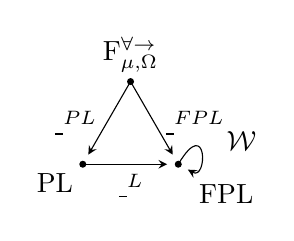
\begin{tikzpicture}[scale=.7, ->, >=stealth]
    % Coordinates for triangle vertices
    \coordinate (A) at (0,1);            % Top: Source Language
    \coordinate (B) at (-0.866,-0.5);    % Bottom left: Logic A
    \coordinate (C) at (0.866,-0.5);     % Bottom right: Logic B
    % Draw dots and labels
    \filldraw (A) circle (1.5pt) node[above] {F$_{\mu,\Omega}^{\forall\to}$};
    \filldraw (B) circle (1.5pt) node[below left] {PL};
    \filldraw (C) circle (1.5pt) node[below right=4pt] {FPL};
    % Arrows with labels and slight offset for arrowhead visibility
    \draw[->, shorten >=4pt] (A) -- (B) node[midway, left] {$\den{\_}^{PL}$};
    \draw[->, shorten >=4pt] (A) -- (C) node[midway, right] {$\den{\_}^{FPL}$};
    \draw[->, shorten >=4pt] (B) -- (C) node[midway, below] {$\den{\_}^L$};
    % Self-loop on Logic B, label offset to avoid overlap
    \draw[->, shorten >=4pt] (C) .. controls (1.4,0.4) and (1.4,-0.8) .. (C)
  node[pos=0.5, right=6pt, yshift=4pt] {$\mathcal{W}$};
  \end{tikzpicture}
  \caption{Translations}
  \label{fig:translations}
\end{figure}



\subsection{Embedding \source in \pl\;\& \fpl}\label{sec:SourceToPL}
\begin{itemize}
  \item explain: $\den{\_}^B := \den{\_}^L \circ \den{\_}^A$
  %\item \eric{TODO: remove exists}
\end{itemize}
We embed \source in \pl\; using the standard CBV-to-CBPV translation\cite{CBPV} as a guide. One notable difference is the handling of our polymorphic, multi-argument function type. Rather than introducing intermediate thunks at every type and term abstraction, we only introduce one top level thunk. \eric{TODO: rethink motivation for the polymorphic multi-arg type and its translation}
\eric{omit the full figure, provide a fragment}
% i think the issue is that thunks were introduced between all type abstractions
% then we'd have a hard time proving..

%\[ \Lambda[](f : \forall[X,Y].(X)\to\mathbb{B}).f = \Lambda[](f : \forall[X,Y].(X)\to\mathbb{B}).\Lambda[X,Y]().f[X,Y]
%  \]


\begin{figure}[H]
\centering
\scriptsize
\begin{align*}
\den{\Gamma \vdash X} &= X \\
\den{\Gamma \vdash \mathbb{B}} &= \mathbb{B} \\
\den{\Gamma \vdash \mathbb{N}} &= \mathbb{N} \\
\den{\Gamma \vdash A\times A'} &= \den{\Gamma \vdash A}\times \den{\Gamma \vdash A'} \\
%\den{\Gamma \vdash \exists X.A} &= \exists X.UF(\den{\Gamma ,X\vdash A})
\end{align*}
\[
\den{\Gamma \vdash \forall[\overrightarrow{X}_n].(\overrightarrow{A}_m)\to A'} 
= U\Bigl(\forall X_1\cdots X_n.\,(\den{\Gamma,\overrightarrow{X}\vdash A_1}, \ldots, \den{\Gamma,\overrightarrow{X}\vdash A_m}) \to F\den{\Gamma,\overrightarrow{X}\vdash A'}\Bigr)
\]
\caption{Type Translation: \source to \pl}
\end{figure}



\begin{figure}[H]
  \centering
  \scriptsize
\begin{align*}
  \den{\Gamma \vdash x}_c &= ret\;x \\
  \den{\Gamma \vdash true}_c &= ret\; true\\
  \den{\Gamma \vdash fasle}_c &= ret\; false\\
  \den{\Gamma \vdash rec_{\mathbb{B}}\;M \; \{N,N'\}}_c &= b \leftarrow \den{\Gamma \vdash M}_c;\; rec_{\mathbb{B}}\; b \; \{\;\den{\Gamma \vdash N}_c|\;\den{\Gamma \vdash N'}_c\}\\
  \den{\Gamma \vdash z}_c &= ret\;z\\
  \den{\Gamma \vdash s \;M}_c &= x \leftarrow \den{\Gamma \vdash M}_c;\; ret(s \; x)\\
  \den{\Gamma \vdash rec_{\mathbb{N}}\;M \; \{N \;|\; x:A.\; N'\}  : A}_c &= n \leftarrow \den{\Gamma \vdash M}_c;\\
  &\quad rec_{\mathbb{N}}\;n\; \{\den{\Gamma \vdash N}_c \;|\; r: U\den{\Gamma \vdash A}. x \leftarrow force \;r; \; \den{\Gamma,x \vdash N'}_c\}\\
  \den{\Gamma \vdash \Omega_A : A}_c &= \Omega_{FA}\\
  \den{\Gamma \vdash \mu x.M : A}_c &= fix[FA](thunk(\lambda r : UF\den{\Gamma \vdash A}. x \leftarrow force\;r;\; \den{\Gamma,x \vdash M}_c)\\
  \den{\Gamma \vdash (M,N)}_c &=\\
  &\;\;\;\; x \leftarrow \den{\Gamma \vdash M}_c;\\
  &\;\;\;\; y \leftarrow \den{\Gamma \vdash N}_c;\\
  &\;\;\;\; ret (x,y)\\
  \den{\Gamma \vdash rec_\times\;M \;\{x,y.\; N\}}_c &= m \leftarrow \den{\Gamma \vdash M}_c;\; rec_\times\;m\;\{x,y.\; \den{\Gamma,x,y\vdash N}_c\}\\
  \den{\Gamma \vdash \Lambda[\overrightarrow{X}_n](\overrightarrow{x}_m).M}_c &= 
  ret(thunk(\\
  &\Lambda X_1.\Lambda X_2.\cdots\Lambda X_n.\\ 
  &\lambda(x:\den{\Gamma,\overrightarrow{X}_n \vdash A_1}).\cdots \lambda(x_m: \den{\Gamma,\overrightarrow{X}_n \vdash A_m}).\\
  &\den{\Gamma ,\overrightarrow{X}_n,\overrightarrow{x}_m\vdash M}_c))\\
  \den{\Gamma \vdash M[\overrightarrow{A}_n](\overrightarrow{M}_m)}_c &= \\
  &m \leftarrow \den{\Gamma \vdash M}_c;\\
  &m_1 \leftarrow \den{\Gamma \vdash M_1}_c;\\
  &\cdots\\
  &m_m \leftarrow \den{\Gamma \vdash M_m}_c;\\
  &(force \;m)\den{\Gamma \vdash A_1}\cdots\den{\Gamma \vdash A_n}(m_1)\cdots(m_m)
  \end{align*}
  \caption{Term Translation: \source to \pl}
\end{figure}


\subsection{Term Language Translation: \pl\;to \fpl}

\eric{only present fragment of translaiton, full translation in appendix}
Here we introduce the backbone of our proof translation which is the term language translation (\cref{fig:TypeTranslationPLFPL},\cref{fig:TermTranslationPLFPL}) between \pl\; and \fpl. 
\subsubsection{Translating $\forall X. \underline{B}$}\label{sec:TranslateForall}
At the core of this translation, as alluded to in \cref{sec:OSum}, is interpretation of $\forall X. \underline{B}$ as \textit{fresh universal quantification} $\forall X. Case\:X \to \underline{B}$. By freshness, we mean to enforce an invariant that all case symbols passed into a universal type are freshly allocated. To demonstrate how this invariant enforces parametric behavior in the presence of $OSum$ and $Case$, consider the following:
\begin{align*}
  &eq_{\sigma_{\mathbb{B}}} : \forall X. Case\;X \to F \mathbb{B}\\
  &\sigma_{\mathbb{B}}: Case\;\mathbb{B}\vdash eq_{\sigma_{\mathbb{B}}} := \Lambda X. \lambda \sigma_X: Case\;X .rec_{OSum}\; (inj_{\sigma_{\mathbb{B}}} true),\sigma_X \; \{x.\;ret\;true\;|\; ret\;false\} 
\end{align*}
The term $eq_{\sigma_{\mathbb{B}}}$ is a case equality test comparing any given $\sigma_X:Case\:X$ to a fixed $\sigma_{\mathbb{B}}:Case\;\mathbb{B}$. As any case symbol is only associated with one type, it is clear to see that $eq_{\sigma_{\mathbb{B}}}$ does not behave parametrically. Note that by ensuring $eq_{\sigma_{\mathbb{B}}}[\mathbb{B}]$ is only ever passed \text{fresh} cases, uniformity is restored.
\begin{align*}
  eq_{\sigma_{\mathbb{B}}}[A](\sigma_A) &\leadsto_{\beta} ret\;false \quad\text{where } A\neq \mathbb{B}\\
  eq_{\sigma_{\mathbb{B}}}[\mathbb{B}](\sigma_{\mathbb{B}}) &\leadsto_{\beta} ret\;true\\
  \sigma_{\mathbb{B}}' \leftarrow new_{\mathbb{B}};eq_{\sigma_{\mathbb{B}}}[\mathbb{B}](\sigma_{\mathbb{B}}') &\leadsto_{\beta} ret\;false\quad\\
\end{align*} 

Via $\den{\_}^L$, any type application in \pl\;allocates a new case symbol, any type abstraction additionally abstracts over a case symbol, and any value type variable in the context has an associated case symbol. It is crucial to note that the case symbol introduced in the translation of type abstraction is not used in the body of the type lambda, a property we will use in our notion of \textit{obliviousness}. Computation type abstraction and application, which are used to church encode $F$ and are not modified. There is no need to do so as they are not within the codomain of $\den{\_}^{PL}$. As the next section will demonstrate, $\den{\_}^L$ alone is not sufficient to enforce the fresh case invariant. 


\begin{figure}[H]
  \centering
  \scriptsize
  % Left column: Context + Type
  \begin{minipage}[t]{0.48\textwidth}
    \[
    \begin{aligned}
      &\textbf{Context:} \\
      \den{\emptyset }^L_{ctx} &= \emptyset \\
      \den{\Gamma,X  }^L_{ctx} &= \den{\Gamma }^L_{ctx} \;, X,\colorbox{lightgray}{$\sigma_X: Case\:X$} \\
      \den{\Gamma,\underline{X}  }^L_{ctx} &= \den{\Gamma }^L_{ctx}\; , \underline{X} \\
      \den{\Gamma, x : A }^L_{ctx} &= \den{\Gamma }^L_{ctx}\; , x : \den{\Gamma \vdash A}^L_{ty} \\[0.5em]
      &\textbf{Types:} \\
      \denLty{\Gamma \vdash \mathbb{B}} &= \mathbb{B} \\
      \denLty{\Gamma \vdash \mathbb{N}} &= \mathbb{N} \\
      \denLty{\Gamma \vdash X} &= X \\
      \denLty{\Gamma \vdash U\underline{B}} &= U \denLty{\Gamma \vdash \underline{B}} \\
      \denLty{\Gamma \vdash A \times A'} &= \denLty{\Gamma \vdash A} \times \denLty{\Gamma \vdash A'} \\
      \denLty{\Gamma \vdash \underline{X}} &= \underline{X} \\
      \denLty{\Gamma \vdash Obs} &= Obs \\
      \denLty{\Gamma \vdash A \rightarrow \underline{B}} &= \denLty{\Gamma \vdash A} \rightarrow \denLty{\Gamma \vdash \underline{B}} \\
      \colorbox{lightgray}{$\denLty{\Gamma \vdash \forall X . \underline{B}}$} &= \colorbox{lightgray}{$\forall X. Case \;X \rightarrow \denLty{\Gamma,X \vdash \underline{B}}$} \\
      \denLty{\Gamma \vdash \forall \underline{X}. \underline{B}} &= \forall \underline{X}. \denLty{\Gamma,\underline{X} \vdash \underline{B}}
    \end{aligned}
    \]
  \end{minipage}\hspace{2em}%
  % Right column: Values + Computations
  \begin{minipage}[t]{0.48\textwidth}
    \[
    \begin{aligned}
      &\textbf{Values:} \\
      \den{\Gamma \vdash x} &= x \\
      \den{\Gamma \vdash true} &= true \\
      \den{\Gamma \vdash false} &= false \\
      \den{\Gamma \vdash z} &= z \\
      \den{\Gamma \vdash s V} &= s \den{\Gamma \vdash V} \\
      \den{\Gamma \vdash thunk\;M} &= thunk \; \den{\Gamma \;|\; \cdot \vdash M} \\
      \den{\Gamma \vdash (V,W)} &= (\den{\Gamma \vdash V}, \den{\Gamma \vdash W}) \\[0.5em]
      &\textbf{Computations:} \\
      \den{\Gamma \vdash rec_{\mathbb{B}}\;V \{M\;|\;N\}} &= rec_{\mathbb{B}}\;\den{\Gamma \vdash V} \;\{\den{\Gamma \vdash M}\;|\;\den{\Gamma \vdash N}\} \\
      \den{\Gamma \vdash rec_{\mathbb{N}}\;V\;\{M \;|\; x. N\}} &= rec_{\mathbb{N}}\;\den{\Gamma \vdash V} \;\{\den{\Gamma \vdash M}\;|\;x. \den{\Gamma, x \vdash N}\} \\
      \den{\Gamma \vdash fix} &= fix \\
      \den{\Gamma \vdash force \;V} &= force\;\den{\Gamma \vdash V} \\
      \den{\Gamma \vdash hault\;V} &= hault\;\den{\Gamma \vdash V} \\
      \den{\Gamma \vdash \lambda x :A. M} &= \lambda x:\den{\Gamma \vdash A}. \den{\Gamma, x : A \vdash M} \\
      \den{\Gamma \vdash MV} &= \den{\Gamma \vdash M}\den{\Gamma \vdash V} \\
      \colorbox{lightgray}{$\den{\Gamma \vdash \Lambda X. M}$} &= \colorbox{lightgray}{$\Lambda X. \lambda \sigma : Case\;X. \den{\Gamma,X \;|\;\Delta \vdash M}$} \\
      \colorbox{lightgray}{$\den{\Gamma \vdash M[A]}$} &= \colorbox{lightgray}{$\sigma \leftarrow new_{\den{\Gamma \vdash A}}; \den{\Gamma \;|\;\Delta \vdash M}[\den{\Gamma \vdash A}](\sigma)$} \\
      \den{\Gamma \vdash \Lambda \underline{X}.M} &= \Lambda \underline{X}. \den{\Gamma , \underline{X} \vdash M} \\
      \den{\Gamma \vdash M[\underline{B}]} &= \den{\Gamma \vdash M}[\den{\Gamma \vdash \underline{B}}] \\
      \den{\Gamma \vdash rec_\times \;V \;\{x,y.\;M\}} &= rec_\times \;\den{\Gamma \vdash V}\;\{x,y.\; \den{\Gamma, x,y \vdash M}\}
    \end{aligned}
    \]
  \end{minipage}
  \caption{Translation of Contexts, Types, Values, and Computations: \pl to \fpl}
  \label{fig:TranslationPLFPL_merged}
\end{figure}



\subsection{Wrapping}\label{sec:Wrap}
%\begin{itemize}
  %\item explain: interesting case, $\forall X.\underline{B}$
  %\item example: demonstrate the protection wrapping provides (use \href{https://publish.obsidian.md/2025/PhD/Shared/Parametricity+Logic/Case+Studies/Deep+Eta}{this} example?) 
  %\item explain: why we get rid of polarity
  %\item remark: on usage of complex values?
  %\item \eric{TODO: remove exists}
%\end{itemize}
The reader may notice that $eq_{\sigma_{\mathbb{B}}}$ will never be in the codomain of $\den{\_}^{FPL}$ and question why we should be concerned about similar misbehaved terms. To answer this, let us consider the interaction between the ambient \textit{environment} and open terms in \pl\;and \fpl.
\[
  f : U(\forall X.F \mathbb{B}) \vdash_{PL} (force\;f) = \Lambda X. (force\;f)[X]
\]
In \pl, the equation above is simply proved using the $\eta$ equality for type $\forall X. F \mathbb{B}$. 
\[
  f : U(\forall X.Case\;X \to F \mathbb{B}) \vdash_{FPL} (force\;f) = \Lambda X. \lambda \sigma_X. \sigma \leftarrow new_X;(force\;f)[X]\sigma
\]
However, in \fpl, if we try to use $\eta\forall$, $\eta\lambda$, and congruence rules, we arrive at: 
\[
  f : U(\forall X.Case\;X \to F \mathbb{B}),X,\sigma_X \vdash_{FPL} (force\;f)[X]\sigma_X = \sigma \leftarrow new_X;(force\;f)[X]\sigma
\]
Note that variable $f$ is not limited to ranging over terms in the codomain of $\den{\_}^{FPL}$. If we consider the environment an adversary, it can provide values which do not behave parametrically. In this case, take $X\mapsto \mathbb{B}, \sigma_X \mapsto \sigma_\mathbb{B}, f \mapsto thunk(eq_{\sigma_{\mathbb{B}}})$ which, as we saw in \cref{sec:TranslateForall}, results in inequal terms.
Generally, unguarded type applications, or failures of our fresh case invariant, can result in inequalities and broken proofs.

Niels et al.\cite{NonParam} solve this issue using a specialized deep $\eta$ expansion, which they call \textit{wrapping}, to surface and guard all type applications. We adapt a simplified version(\cref{fig:wrapping}) of their wrapping strategy to preserve equalities in our proof translation. However, wrapping introduces complications in our proof translation as we demonstrate in \cref{d}.

\begin{figure}[H]
  \centering
  \scriptsize
  % Left column: Base types + product + U
  \begin{minipage}[t]{0.48\textwidth}
    \[
    \begin{aligned}
      &\mathcal{W} _X(t) := t \\
      &\mathcal{W} _\mathbb{B}(t) := t \\
      &\mathcal{W} _\mathbb{N}(t) := t \\
      &\mathcal{W} _{Obs}(t) := t \\
      &\mathcal{W} _{A \times A'}(t) := rec_\times \;t\;\{x,y.\; (\mathcal{W} _A(x),\mathcal{W} _{A'}(y))\} \\
      &\mathcal{W}_{U\underline{B}}(t) := thunk(\mathcal{W} _{\underline{B}}(force\;t)) \\
    \end{aligned}
    \]
  \end{minipage}\hspace{2em}%
  % Right column: Functions + forall + contexts
  \begin{minipage}[t]{0.48\textwidth}
    \[
    \begin{aligned}
      &\mathcal{W}_{\underline{X}}(t) := t\\
      &\mathcal{W} _{A \rightarrow \underline{B}}(t) := \lambda(x:A).\mathcal{W}_{\underline{B}}(t(\mathcal{W}_A(x))) \\
      &\colorbox{lightgray}{$\mathcal{W}_{\forall X.\underline{B}}(t) := 
      \Lambda X.\lambda \sigma_X.  \mathcal{W}_{\underline{B}}(\sigma_X'\leftarrow new_X;\;t[X](\sigma_X'))$} \\
      &\mathcal{W}_{\forall \underline{X}.\underline{B}}(t) := \Lambda \underline{X}.\mathcal{W}_{\underline{B}}(t[\underline{X}]) \\\\
      &\mathcal{W}_\Gamma(t) := t[\mathcal{W}_{A_1}(x_1)/x_1,\cdots,\mathcal{W}_{A_n}(x_n)/x_n] \\
      &\quad \text{ where } x_1:A_1,\cdots,x_n:A_n \in \Gamma
    \end{aligned}
    \]
  \end{minipage}
  \caption{Wrapping}
  \label{fig:wrapping}
\end{figure}


\section{Logics}\label{sec:Logics}
\begin{itemize}
  \item explain: rules of Logic A
  \item explain: relational interpretation of types (including Case,OSum)
  \item explain: IEP axiom
\end{itemize}
\eric{this section needs more exposition. Nothing fancy, just explain the parts of the logic and provide an example to conclude}
Here we present the parametricity logics \pl\;and \fpl.

\subsection{Core}
\eric{cite PE, mention influence}
Both \pl\;and \fpl\;are based on a higher order logic, permitting quantification over predicates and relations(\cref{fig:Props}). The distinction between value and computations types is extended to our logics as well. Here we have separate classes of value and computation predicates and relations. Propositions (\cref{fig:PropFormation}) and relations (\cref{fig:RelFormation}) are judged to be well-formed with respect to a context, $\Gamma$, of types and terms and a context, $\Theta$, of value and computation relations.  Proof sequents are of the form $\Gamma ; \Theta \;|\; \Phi \vdash \phi$ where $\Phi$ is a context of well-formed propositions in context $\Gamma; \Theta$. A fragment of the derivation rules appear in \cref{fig:Derivation}. 

In addition to the derivation rules, our logic provides a number of rules that are useful in proving parametricity theorems. First, many parametricy proofs boil down to creatively picking a relation. Frequently, these relations are based on the graph of some function. As an example, take the function $even : \mathbb{N} \to F \mathbb{B}$ used to establish a relation $\langle even \rangle : Rel_v[\mathbb{N},\mathbb{B}]$ between $\mathbb{N}$ and $\mathbb{B}$. This can be constructed using the graph rule. 
\begin{figure}[H]
  \centering  
  \scriptsize
  % First proof tree
  \begin{minipage}[b]{0.48\textwidth}
    \centering
    \begin{prooftree}
      \AxiomC{}
      \RightLabel{asm}
      \UnaryInfC{$\Gamma\;|\; \cdot \vdash f : A \rightarrow F A'$}
      \RightLabel{weaken}
      \UnaryInfC{$\Gamma,x : A \;|\; \cdot \vdash f : A \rightarrow F A'$}
      \AxiomC{}
      \UnaryInfC{$\Gamma, x : A \vdash x : A$}
      \BinaryInfC{$\Gamma,x : A \;|\; \cdot \vdash f(x) : F A'$}
      \AxiomC{}
      \UnaryInfC{$\Gamma,y : A' \vdash y : A'$}
      \UnaryInfC{$\Gamma,y : A'  \;|\; \cdot \vdash ret \; y : FA'$}
      \BinaryInfC{$\Gamma ; \Theta\vdash (x : A, y: A'). f(x) =_{FA} ret \; y : Rel_v[A,A']$}
      \dashedLine
      \UnaryInfC{$\Gamma ; \Theta \vdash \langle f \rangle : Rel_v[A,A']$}
    \end{prooftree}
    %\caption*{Detailed derivation}
  \end{minipage}\hfill
  $\leadsto$
  % Second proof tree
  \begin{minipage}[b]{0.3\textwidth}
    \centering
    \begin{prooftree}
      \AxiomC{$\Gamma \;|\; \cdot \vdash f : A \rightarrow FA'$}
      \RightLabel{graph$\lambda_c$}
      \UnaryInfC{$\Gamma ; \Theta \vdash \langle f \rangle : Rel_v[A,A']$}
    \end{prooftree}
    %\caption*{Graph rule summary}
  \end{minipage}

  \caption{Graph Rule}
  \label{fig:Graph}
\end{figure}



We provide induction principles for $\mathbb{B}$ and $\mathbb{N}$ which are useful in proving propositions such as $\forall n : \mathbb{N}, b : \mathbb{B}. \langle even \rangle (n,b) \implies \langle even \rangle(2 + n,b)$. As \pl\;and \fpl\;are both programming logics, we include the equational theories (\cref{fig:EquationalTheory}) of the term languages, including congruence rules and derivable rules about function extensionality. 




% small section on what rules are useful to prove parametricity theorems
% maybe a example parametricity proof ?
%\eric{equal relation, graph relations}

%\eric{induction rules for bool and nat}

%\eric{equational theory  + congruence rules, derivable fun ext rules}

%\eric{congruence rules for ret and bind are derivable}

\subsection{Parametricity Axiom}
Thus far, we have set up a higher order programming logic. In order to reason about parametricity, we need to define a relational interpretation of types and add an axiom schema.

%\subsubsection{Relational Interpretation of Types}
%\subsubsection{Identity Extension Principle}
% relational interpretation of F 
% what about Case and OSum? we leave them opaque in the logic
The relational interpretation of types is given in \cref{fig:RelInterp}. The synatx "$\mathcal{V}[A]_{\rho,\underline{\rho}}$"  can be seen as a \textit{marco} which, given a value type $A$, unfolds to a value relation $Rel_v[A',A'']$. Relation environments, $\rho,\underline{\rho}$, consists of a mapping $X\mapsto (Y,Z,R : Rel[Y,Z])$ from type variable $X$ to a tuple of two types $Y,Z$ and a relation $R : Rel[Y,Z]$. We use $A[\rho_L]$ to denote a type substitution which replaces every type variable $X$ in $A$ with the corresponding type given by the first element of tuple $\rho(X)$. \eric{more context, why introduce this, what are the interesting cases}

In order to make use of the relational interpretation of types, we employ an axiom schema for the \textit{Identity Extension Principle}.

\begin{definition}
  Identity Extension Principle. For all types $A$, we have:
  \begin{align*}
    &  \Gamma ; \Theta \;|\; \Phi \vdash \forall x,y : A. \mathcal{V}[A]_{\overrightarrow{eq},\underline{\overrightarrow{eq}}}(x,y) \iff x =_A y  \\ 
  \end{align*}
\end{definition}

To understand the utility of this principle, we can observe what it says for the universal type. For any $M,N : \forall X.\underline{B}$:
\[
  \forall Y,Z,R:Rel_v[Y,Z].\mathcal{C}[\underline{B}]_R(M[Y],N[Z]) \iff M =_{\forall X. \underline{B}} N
\]


\subsection{Parametricity Proof}
\eric{rename section, demonstrate that this logic can actually prove parametricty theorems}
Swap Proof in \pl

\begin{figure}[h]
  \centering
  \eric{predicates}

  \begin{align*}
    \phi :=&\; \bot\;|\;V=_{A}W \;|\; M=_{\underline{B}}N \;|\; R(V,W) \;|\; \underline{R}(M,N) \;|\; 
    \\
    &\; \phi \land \psi \;|\; \phi \lor \psi \;|\; \phi \implies \psi \;|\; \exists \square.\phi \;|\; \forall \square .\phi \\ 
  %  &\;\forall(x : A).\phi \;|\; \forall X . \phi \;|\; \forall \underline{X}.\phi \;|\; \forall R. \phi \;|\; \forall \underline{R}. \phi \;|\; 
   % &\; \exists(x : A).\phi \;|\; \exists X . \phi \;|\; \exists \underline{X}.\phi \;|\; \exists R. \phi \;|\; \exists \underline{R}.\phi\\
    & \square \in \{x:A,X,\underline{X},R:Rel_v[A,A'],\underline{R}:Rel_c[\underline{B},\underline{B}']\}
    \end{align*}
  \caption{Propositions}
  \label{fig:Props}
\end{figure}


\begin{figure}[h]
  \centering 
  \scriptsize
  \begin{mathpar}
    \inferrule
      { \Gamma \vdash V : A \\ \Gamma \vdash W : A }
      { \Gamma;\Theta \vdash V =_{A} W : Prop }
    
    \inferrule
      { \Gamma \;|\; - \vdash M : \underline{B} \\ \Gamma \;|\; - \vdash N : \underline{B} }
      { \Gamma;\Theta \vdash M =_{\underline{B}} N : Prop }
    
    \inferrule
      { \Gamma \vdash V : A \\ \Gamma \vdash W : A' \\ R : Rel_v[A,A'] \in \Theta }
      { \Gamma;\Theta \vdash R(V,W) : Prop }
    
    \inferrule
      { \Gamma \;|\; - \vdash M : \underline{B} \\ \Gamma \;|\; - \vdash N : \underline{B'} \\
        \underline{R} : Rel_c[\underline{B},\underline{B'}] \in \Theta }
      { \Gamma;\Theta \vdash \underline{R}(M,N) : Prop }
    
    \inferrule
      { \Gamma;\Theta \vdash \phi : Prop \\ \Gamma;\Theta \vdash \psi : Prop }
      { \Gamma;\Theta \vdash \phi \square \psi }
    \quad (\square \in \{\land,\lor,\implies\})
    
    \inferrule
      { \Gamma,x : A;\Theta  \vdash \phi : Prop }
      { \Gamma;\Theta \vdash \forall (x : A). \phi : Prop }
    
    \inferrule
      { \Gamma;\Theta \vdash \phi : Prop }
      { \Gamma;\Theta \vdash \forall X . \phi : Prop }
    %\quad (X \notin frv(\Theta,\Gamma))
    
    \inferrule
      { \Gamma;\Theta, R \vdash \phi : Prop }
      { \Gamma;\Theta \vdash \forall (R : Rel_v[A,B]). \phi : Prop }
    \end{mathpar}
    
    
  \caption{Proposition Formation Rules Fragment}
  \label{fig:PropFormation}
\end{figure}


\begin{figure}[h]
  \centering 
  \scriptsize
  \begin{mathpar}
    % Equality Prop
    \inferrule
      { \Gamma , x : A \;|\;  \cdot \vdash V : C \\ \Gamma , y : A' \;|\;  \cdot \vdash W : C }
      { \Gamma ; \Theta \vdash (x : A, y : A'). V=_C W : Rel_v[A,A'] }
    
    \inferrule
      { \Gamma \;|\; x : \underline{B}\vdash M : \underline{C} \\ \Gamma  \;|\;  y : \underline{B'} \vdash N : \underline{C} }
      { \Gamma ; \Theta \vdash (x : \underline{B}, y : \underline{B'}). M=_{\underline{C}} N : Rel_c[\underline{B},\underline{B'}] }
    

    
    % Binary Connectives 
    \inferrule
      { \Gamma ; \Theta \vdash (x :A, y : C).\phi : Rel_=[A,C] \\ \Gamma ; \Theta \vdash (x :A, y : C).\psi : Rel_=[A,C] }
      { \Gamma; \Theta \vdash (x :A, y : C). \phi \land \psi : Rel_=[A,C] }

      \inferrule
      { \Gamma ; \Theta \vdash \phi : Prop \\ \Gamma ; \Theta \vdash (x :A, y : C).\psi : Rel_=[A,C] }
      { \Gamma; \Theta \vdash (x :A, y : C). \phi \implies \psi : Rel_=[A,C] }
    
    % Quantifier Connectives - Terms
    \inferrule
      { \Gamma, x : C ; \Theta \vdash (x : A, y : B). \phi : Rel_=[A,B] }
      { \Gamma ; \Theta \vdash (x : A, y : B). \forall x  : C. \phi : Rel_=[A,B] }
    
    % Quantifier Connectives - Types
    \inferrule
      { \Gamma ; \Theta \vdash (x : A, y : B). \phi : Rel_=[A,B] }
      { \Gamma ; \Theta \vdash (x : A, y : B). \forall X  . \phi : Rel_=[A,B] }
    
    % Quantifier Connectives - Relations (only value relations)
    \inferrule
      { \Gamma, \Theta, R: Rel_=[C,C'] \vdash (x : A, y : B). \phi : Rel_-[A,B] }
      { \Gamma ; \Theta \vdash (x : A, y : B). \forall R: Rel_=[C,C']  . \phi : Rel_-[A,B] }
    \end{mathpar}
    
  \caption{Relation Formation Rules Fragment}
  \label{fig:RelFormation}
\end{figure}

\begin{figure}[h]
  \centering
  \scriptsize
  \begin{mathpar}
    % Ex falso
    \inferrule
      { \Gamma;\Theta \;|\; \Phi \vdash \bot }
      { \Gamma ; \Theta \;|\; \Phi \vdash \phi }
    
    % Equality - reflexivity
    \inferrule
      { \Gamma \vdash V : A }
      { \Gamma ; \Theta \;|\; \Phi \vdash V =_{A} V }
    
    % Equality - substitution
    \inferrule
      { \Gamma;\Theta\; |\; \Phi \vdash V =_A W \\ \Gamma;\Theta \;|\;\Phi \vdash \phi[V/x] }
      { \Gamma;\Theta\;|\; \Phi \vdash \phi[W/x] }
    
    % Conjunction introduction
    \inferrule
      { \Gamma;\Theta \;|\; \Phi \vdash \phi \\ \Gamma;\Theta \;|\; \Phi \vdash \psi }
      { \Gamma;\Theta \;|\; \Phi \vdash \phi \land \psi }
    
    % Conjunction elimination
    \inferrule
      { \Gamma;\Theta \;|\; \Phi \vdash \phi \land \psi }
      { \Gamma;\Theta \;|\; \Phi \vdash \phi }
    
    % Universal quantifier (type) introduction
    \inferrule
      { \Gamma,X;\Theta \;|\; \Phi \vdash \phi }
      { \Gamma;\Theta \;|\; \Phi \vdash \forall X . \phi }
    \quad (X \notin ftv(\Theta, \Gamma, \Phi))
    
    % Universal quantifier (type) elimination
    \inferrule
      { \Gamma;\Theta \;|\; \Phi \vdash \forall X . \phi }
      { \Gamma;\Theta \;|\; \Phi \vdash \phi[A/X] }
    
    % Universal quantifier (relation) introduction
    \inferrule
      { \Gamma;\Theta,R \;|\;\Phi \vdash \phi }
      { \Gamma;\Theta \;|\;\Phi \vdash \forall (R : Rel_v[A,B]). \phi }
    
    % Universal quantifier (relation) elimination
    \inferrule
      { \Gamma;\Theta \;|\; \Phi \vdash \forall (R : Rel_v[A,B]). \phi \\ \Gamma;\Theta  \vdash (x : A, y: B). \psi : Rel_v[A,B] }
      { \Gamma;\Theta \;|\; \Phi \vdash \phi[\psi[M/x,N/y]/R(M,N)] }
    \end{mathpar}
    
  \caption{Derivation Rules Fragment}
  \label{fig:Derivation}
\end{figure}


\begin{figure}[H]
  \centering
  \scriptsize
  \eric{Obs}
  \eric{thunk computation bindings}
  \eric{highlight Case, OSum}
  \begin{align*}
    &\mathcal{V}[X]_{\rho,\underline{\rho}} = \rho(X)\\
    &\mathcal{V}[\mathbb{B}]_{\rho,\underline{\rho}} = (x:\mathbb{B}, y: \mathbb{B}). \; x = y\\
    &\mathcal{V}[\mathbb{N}]_{\rho,\underline{\rho}} =(x:\mathbb{N}, y: \mathbb{N}). \; x = y\\
    &\mathcal{V}[U\underline{B}]_{\rho,\underline{\rho}} = (x : U\underline{B}[\rho_L,\underline{\rho_L}], y :U\underline{B}[\rho_R,\underline{\rho_R}] ). \mathcal{C}[\underline{B}]_{\rho,\underline{\rho}}(force\;x, force\; y)
    \\
    &\mathcal{V}[A\times A']_{\rho,\underline{\rho}} = (p_1 : (A\times A')[\rho_L,\underline{\rho_L}],p_2 : (A\times A')[\rho_R,\underline{\rho_R}]).\\
    &\quad  
    \exists e_1:A[_L],e_2:A'[_L],e_3:A[_R],e_4: A'[_R].\\
    &\quad \quad p_1 = (e_1,e_2) \land p_2 = (e_3,e_4) \land \mathcal{V}[A]_{\rho,\underline{\rho}}(e_1,e_3) \land \mathcal{V}[A']_{\rho,\underline{\rho}}(e_2,e_4)
    \\
    \\
    &\mathcal{C}[\underline{X}]_{\rho,\underline{\rho}} = \underline{\rho}(\underline{X})\\
    &\mathcal{C}[Obs_{\mathbb{B}}]_{\rho,\underline{\rho}} = (x: Obs_{\mathbb{B}},y: Obs_{\mathbb{B}}).\\
    &\quad \exists b_1,b_2 . x = hault \; b_1 \land y = hault \;b_2 \land  \mathcal{V}[\mathbb{B}](b_1,b_2)\\
    &\mathcal{C}[A\rightarrow \underline{B}]_{\rho,\underline{\rho}} = (f : (A \rightarrow \underline{B})[\rho_L,\underline{\rho_L}],g : (A \rightarrow \underline{B})[\rho_R,\underline{\rho_R}]).\\&\;\;\;\;\;\;\;\forall x : A[\rho_L,\underline{\rho_L}], y: A[\rho_R,\underline{\rho_R}].\mathcal{V}[A]_{\rho,\underline{\rho}}(x,y) \implies \mathcal{C}[\underline{B}]_{\rho,\underline{\rho}}(fx,gy)\\
    &\mathcal{C}[\forall X. \underline{B}]_{\rho,\underline{\rho}} = (f : \forall X.\underline{B}[\rho_L,\underline{\rho_L}],g : \forall X.\underline{B}[\rho_R,\underline{\rho_R}]). \\&\;\;\;\;\;\;\;
    \forall Y,Z,R:Rel_v[Y,Z]. \mathcal{C}[\underline{B}]_{\rho,R,\underline{\rho}}(f[Y],g[Z])
    \\
    &\mathcal{C}[\forall \underline{X}.\underline{B}]_{\rho,\underline{\rho}} = (f : \forall \underline{X}.\underline{B}[\rho_L,\underline{\rho_L}],g : \forall \underline{X}.\underline{B}[\rho_R,\underline{\rho_R}]). \\&\;\;\;\;\;\;\;
    \forall \underline{Y},\underline{Z},\underline{R}:Rel_c[\underline{Y},\underline{Z}]. \mathcal{C}[\underline{B}]_{\rho,\underline{\rho},\underline{R}}(f[\underline{Y}],g[\underline{Z}])
    \end{align*}
    \caption{Relational Interpretation of Types}
  \label{fig:RelInterp}
\end{figure}


\section{Preserving Logical Equivalence}\label{sec:LogicEquiv}
In this section
Here we state our theorem in full detail. The remainder of this section will be dedicated to defining the proof translation and presenting lemmas we think are necessary to prove our result.


\subsection{Obliviousness}\label{sec:Obliv}
Modifying the terms in a proof has consequences. Without any adjustment to our interpretation of propositions, proofs which use $\eta$ expansion for value type abstraction break. Considering the following convoluted proof of $2=2$ in \pl\footnote{Note that $\mathcal{W}[\mathbb{B}]$ is the identity function, so wrapping does not play a role in the translated proof.}.


\begin{figure}[H]
  \centering 
  \footnotesize
  \begin{prooftree}
    \AxiomC{$\vdash 2 : \mathbb{N} $}
    \RightLabel{refl}
    \UnaryInfC{$\vdash 2 = 2$}
    \AxiomC{$f \vdash (force\;f) : \forall X. \underline{B}$}
    \RightLabel{$\eta\forall$}
    \UnaryInfC{$f \vdash (force\;f) = \Lambda X.(force\;f)[X]$}
    \RightLabel{I$\forall_{vtm}$}
    \UnaryInfC{$\vdash \forall f.(force\;f) = \Lambda X.(force\;f)[X]$}
    \RightLabel{I$\land$}
    \BinaryInfC{$\vdash 2 = 2 \land \forall f : U(\forall X. \underline{B}).(force\;f) = \Lambda X. (force\;f)[X]$}
    \RightLabel{E$\land_1$}
    \UnaryInfC{$\vdash 2 = 2$}
    \end{prooftree} 
\end{figure}


The proof statement $2 = 2$ could simply be solved using reflexivity, but our logical equivalence theorem states that we should be able to handle any possible proof of $2=2$, even one which introduces superfluous derivations. Assuming the proposition and derivation translation from \pl\;to \fpl\; do not introduce extra hypotheses, we run into a problem. Specifically, we do not have enough information to prove the rule $\eta\forall$ under translation. Given $\den{\Gamma} \vdash \den{M}: \den{\forall X. \underline{B}}$, show $\den{\Gamma} ; \den{\Theta} \;|\; \den{\Phi} \vdash \den{M} = \den{\Lambda X. M[X]}$ in \fpl. Or, as in our concrete example above:
\begin{figure}[H]
  \centering 
  \footnotesize
  \begin{prooftree}
    \AxiomC{$f : \den{U(\forall X. \underline{B})} \vdash \den{(force\;f)} : \den{\forall X. \underline{B}} $}
    \dashedLine
    \UnaryInfC{$f : U(\forall X. Case\;X \to \den{\underline{B}}) \vdash (force\;f) : \forall X. Case\;X \to \den{ \underline{B}} $}
  
    \UnaryInfC{$?$}
    \UnaryInfC{$f \vdash force\;f = \Lambda X.\lambda \sigma_X. \sigma \leftarrow new_X;(force\;f)[X]\sigma$}
    \dashedLine
    \UnaryInfC{$f \vdash \den{force\;f} = \den{\Lambda X .(force\;f)[X]}$}
    \end{prooftree} 
\end{figure}
Using the rules of \fpl\;to $\eta$ expanding lambdas on the left-hand-side of the equation as well as congruence rules for lambdas yields: 
\begin{equation}
  \label{eqn:Obliv1}
  f,X,\sigma_X \vdash (force\;f)[X]\sigma_X = \sigma \leftarrow new_X;(force\;f)[X]\sigma
\end{equation}
Note that if the variable $f$ was wrapped, then this equation would hold. But, as we saw in the example above, the wrapping \textit{did not cover} $f$. To patch over this issue, we introduce the concept of \textit{obliviousness}. 

%\subsubsection{Obliviousness}
We define obliviousness (\cref{fig:Oblivious}) as a \pl\;type-indexed \textit{logical predicate} over terms in \fpl. An oblivious term is one which cannot use case symbols in any meaningful way. In particular, it is not able to distinguish between a fresh case symbol and one which has already been allocated. Formally, this property is encoded in the obliviousness predicate as an equation in case $\mathcal{O}[\forall X. \underline{B}]$.


\begin{figure}[H]
  \centering
  \scriptsize
  \begin{align*}
    &\mathcal{O}[X]_{\rho}(V :\rho_{ty}(X)) := \rho_{rel}(X)(V)\\
    &\mathcal{O}[\mathbb{B}]_{\rho} (V : \mathbb{B}):= \top \\% V = true \lor V = false\\
    &\mathcal{O}[\mathbb{N}]_{\rho}(V : \mathbb{N}) := \top\\%V = z \lor \exists n : \mathbb{N}. V = s n\\
    &\mathcal{O}[A \times A']_{\rho}(V : \den{A\times A'}^L_{ty}[\rho]) := \exists x_1:\den{A}^L_{ty}[\rho],x_2:\den{A'}^L_{ty}[\rho].\\
    &\quad V = (x_1,x_2) \land \mathcal{O}[A]_{\rho}(x_1) \land \mathcal{O}[A']_{\rho}(x_2)\\
    &\mathcal{O}[U\underline{B}]_{\rho}(V : \den{\underline{B}}^L_{ty}[\rho] )) := \mathcal{O}[\underline{B}]_{\rho}(force\;V)\\
    \\
    & \mathcal{O}[\underline{X}]_{\rho}(V: \rho_{ty}(\underline{X})) := \rho_{rel}(\underline{X})(V)\\
    &\mathcal{O}[A\rightarrow \underline{B}]_{\rho}(M : \den{A \rightarrow \underline{B}}^L_{ty}[\rho]) := \forall\; V :\den{A}^L_{ty}[\rho]. \mathcal{O}[A]_{\rho}(V)\implies \mathcal{O}[\underline{B}]_{\rho}(MV) \\
    &\mathcal{O}[\forall X. \underline{B}]_{\rho}(M :\den{\forall X. \underline{B}}^L_{ty}[\rho]) := \\
    &\quad \forall X,P:Pred[X],\sigma_X:Case\:X.\\
    &\quad \quad \colorbox{lightgray}{$\mathcal{O}[\underline{B}]_{{\rho},P}(M[X](\sigma_X))$} \\
    &\quad \quad \land \colorbox{lightgray}{$M[X](\sigma_X) = (\sigma\leftarrow new_X; M[X](\sigma))$}\\
    &\mathcal{O}[\forall \underline{X}. \underline{B}]_{\rho}(M:\den{\forall \underline{X}. \underline{B}}^L_{ty}[\rho]) := \forall \underline{X},\underline{P}: Pred[\underline{X}].\mathcal{O}[\underline{B}]_{\rho,\underline{P}}(M[\underline{X}]) 
\end{align*}
  \caption{Obliviousness Predicate}
  \label{fig:Oblivious}
\end{figure}

To demonstrate how obliviousness solves our problem, we reconsider \cref{eqn:Obliv1} with an added hypothesis, $H_f$, about the obliviousnes of $f$ in \cref{eqn:Obliv2}. Our hypothesis $H_f$ applied to $X,P_X,\sigma_X$ gives us a proof of obliviousness $\mathcal{O}[\underline{B}]((force\;f)[X]\sigma_X)$ and the exact equation we are trying to prove.

\begin{equation}
  \label{eqn:Obliv2}
  f,X,\sigma_X;\colorbox{lightgray}{$P_X \;|\; H_f : \mathcal{O}[U(\forall X. \underline{B})](f) $} \vdash (force\;f)[X]\sigma_X = \sigma \leftarrow new_X;(force\;f)[X]\sigma
\end{equation}

We define our proof translation making usage of obliviousness.
In order to justify our approach, we prove an \textit{adequacy} theorem in \cref{sec:Adequacy} demonstrating that our usage of obliviousness is sound. While wrapping \fpl\;terms enforces the freshness invariant, it complicates the proof translation by potentially introducing $\eta$ expansions and allocation of fresh cases which modify the terms in a proof. Obliviousness helps here as well by enabling a more compositional approach to proof translation, as we will see in section \cref{sec:ProofTranslation}. 


\subsection{Proposition Translation}\label{sec:PropTranslation}
As we saw in the last section, in order to preserve \pl\;proofs we needed terms to be \textit{oblivious} to case symbols. We introduce obliviousness via the proof translation from \pl\;to \fpl. Here we define a translation $\den{\_}^O$ which enhances the term translation $\den{\_}^L$ by pairing a translated term with a proof of its obliviousness. Additionally, $\den{\_}^O$ adds data to the context required by the definition of obliviousness. Specifically, any term variable $x :A$ in the context has an associated obliviousness hypothesis $H_x : \mathcal{O}[A](x)$ in the proof context and type variables $X/\underline{X}$ are associated with predicates $P/\underline{P}$ so that type variables can be interpreted in the obliviousness predicate. 



\begin{figure}[H]
  \centering
  \scriptsize
  \begin{align*} 
    &\den{\Gamma,x:A}^O := \den{\Gamma}^O,x : \den{A}^L \;|\; \colorbox{lightgray}{$H_x : \mathcal{O}[A](x)$}\\
    &\den{\Gamma,X}^O := \den{\Gamma}^O,X,\sigma_X : Case\;X ; \colorbox{lightgray}{$P : Pred[X]$}\\
    &\den{\Gamma,\underline{X}}^O := \den{\Gamma}^O,\underline{X};\colorbox{lightgray}{$\underline{P} : Pred[\underline{X}]$}\\
    \\
    &\den{\Gamma \vdash_{PL} M : A}^O := \den{\Gamma \vdash_{PL} M : A}^L, \colorbox{lightgray}{$\mathcal{O}[A](\den{M})$} 
  \end{align*}
  \caption{Obliviousness Context and Term Translation}
  \label{fig:d}
\end{figure}

For the invariants on contexts to be preserved, we must adjust the translation of propositions. Quantification over a value $x : A$ introduces an obliviousness hypothesis $\mathcal{O}[A](x)$. Quantification over computation types $\underline{X}$ introduces a predicate $\underline{P}_{\underline{X}}$. Quantification over value types $X$ introduces a predicate $P$ as well as a case symbol $\sigma_X : Case\;X$.

\begin{figure}[H]
  \centering
  \scriptsize
  \begin{align*}
    \den{\Gamma;\Theta\vdash_A \bot}^L_{prop}  &=\; \bot \\
    \den{\Gamma;\Theta\vdash_A V =_A W}^L_{prop} &=\; \den{\Gamma \vdash _AV}^O =_{\den{\Gamma \vdash A}^L_{ty}}  \den{\Gamma \vdash W}^O \\
    \den{\Gamma;\Theta\vdash_A M =_{\underline{B}} N}^L_{prop} &=\;     \den{\Gamma \vdash M}^O =_{\den{\Gamma \vdash \underline{B}}^L_{ty}}   \den{\Gamma  \vdash N}^O \\
    \den{\Gamma;\Theta\vdash_A R(V,W)}^L_{prop} &=\;   \den{\Gamma ;\Theta\vdash _AR}^L_{rel_v}(  \den{\Gamma \vdash V}^O,   \den{\Gamma \vdash W}^O) \\
    %\den{\Gamma;\Theta\vdash_A \underline{R}(M,N)}^L_{prop} &=\;   \den{\Gamma ; \Theta\vdash_A\underline{R}}^L_{rel_c}(  \den{\Gamma \vdash M}^O,   \den{\Gamma \vdash N}^O) \\
    \den{\Gamma;\Theta\vdash_A \phi \land \psi}^L_{prop} &=\;   \den{\Gamma;\Theta\vdash_A \phi}^L_{prop} \land \den{\Gamma;\Theta\vdash_A \psi}^L_{prop} \\
    %\den{\Gamma;\Theta\vdash_A \phi \lor \psi}^L_{prop} &=\;   \den{\Gamma;\Theta\vdash_A \phi}^L_{prop} \lor \den{\Gamma;\Theta\vdash_A \psi}^L_{prop} \\
    %\den{\Gamma;\Theta\vdash_A \phi \implies \psi}^L_{prop} &=\;   \den{\Gamma;\Theta\vdash_A \phi}^L_{prop} \implies \den{\Gamma;\Theta\vdash_A \psi}^L_{prop} \\
    \den{\Gamma;\Theta\vdash_A \forall(x:A).\phi}^L_{prop} &=\;   \forall(x:\den{\Gamma  \vdash A}^L_{ty}).\colorbox{lightgray}{$\mathcal{O}[A](x)\implies$}\den{\Gamma,x : A\;\Theta\vdash_A \phi}^L_{prop} \\
    \den{\Gamma;\Theta\vdash_A \forall X.\phi}^L_{prop} &=\;   \forall X,\colorbox{lightgray}{$P : Pred[X],\sigma_X:Case\;X$}.\den{\Gamma,X;\Theta\vdash_A \phi}^L_{prop}\\
    \den{\Gamma;\Theta\vdash_A \forall \underline{X}.\phi}^L_{prop} &=\;   \forall \underline{X},\colorbox{lightgray}{$\underline{P}:Pred[\underline{X}]$}.\den{\Gamma,\underline{X};\Theta\vdash_A \phi}^L_{prop} \\
    \den{\Gamma;\Theta\vdash_A \forall R:Rel_v[A,A'].\phi}^L_{prop} &=\;   \forall  R:Rel_v[\den{\Gamma \vdash A}^L_{ty},\den{\Gamma \vdash A'}^L_{ty}].\den{\Gamma;\Theta,R:Rel_v[A,A']\vdash_A \phi}^L_{prop}\\
    %\den{\Gamma;\Theta\vdash_A \forall \underlineL_{tm}{R}:Rel_c[\underline{B},\underline{B}'].\phi}^L_{prop} &=\;   \forall \underline{R}:Rel_c[\den{\Gamma \vdash \underline{B}}^L_{ty},\den{\Gamma \vdash \underline{B}'}]^L_{ty}.\den{\Gamma;\Theta,\underline{R}:Rel_c[\underline{B},\underline{B}']\vdash_A \phi}^L_{prop}
    \end{align*}
    \caption{Proposition Translation Fragment}
    \label{fig:PropTranslation}
\end{figure}




  
\subsection{Oblivious Proof Translation}\label{sec:ProofTranslation}
Here we demonstrate the first key theorem (\cref{thm:OblivTranslation}) in our preservation of logical equivalence. This theorem relies on auxiliary lemmas demonstrating that our term and type translations are sound, such as the preservation of typing.

\begin{lemma} $\den{\_}^L$ Preserves well-formedness of types and well-typedness of terms
 % $\forall A \;VType_{PL}. \den{A}^L \;VType_{FPL}$
  \end{lemma}

\begin{proof}
  This is mostly routine. The case for type application is slightly complicated by the need to use typing rules for church encoded bind.
\end{proof}

%\begin{theorem} $\den{\_}^{PL}$ Preserves well-formedness of types and well-typedness of terms
% $\forall A \;VType_{PL}. \den{A}^L \;VType_{FPL}$
%\end{theorem}

%\begin{theorem} $\den{\_}^{FPL}$ Preserves well-formedness of types and well-typedness of terms
  % $\forall A \;VType_{PL}. \den{A}^L \;VType_{FPL}$
%\end{theorem}
  
Here we demonstrate that for any $\Gamma \vdash_{PL} V : A$ we can provide a proof $\den{\Gamma}^O \vdash_{FPL} \mathcal{O}[A](\den{V}^L)$ as demanded by our updated term translation. In other words, obliviousness is a congruence with respect to the typing rules of \pl.
\eric{TODO: this typesetting looks like shit}
\begin{lemma}
  \label{lem:OblivTerm}
  $\Gamma \vdash_{PL} V : A \implies \den{\Gamma}^O \vdash_{FPL} \mathcal{O}[A](\den{V})$
\end{lemma}
\begin{proof}
  By induction on the typing rules of $\mathbf{PL}$. We consider the interesting cases here.
  \paragraph{$Case: \Lambda X. M : \forall X. \underline{B}$}
  \indent

  \quad Given: $\den{\Gamma}^O,X\sigma_X;P_X \vdash \mathcal{O}[\underline{B}](\den{M}^L)$

  \quad Prove: $\den{\Gamma}^O \vdash \mathcal{O}[\forall X. \underline{B}](\den{\Lambda X. M}^L)$

  We have to show $\forall X,P_X,\sigma_X.\mathcal{O}[\underline{B}](\den{\Lambda X.M}^L[X]\sigma_X) \land \den{\Lambda X. M}^L[X]\sigma_X = \sigma \leftarrow new_X;\den{\Lambda X. M}^L[X]\sigma$.
  Here we use the observation that the translation of a type lambda is oblivious, the body $\den{X \vdash M}^L$ does not use $\sigma_X.$ Thus, we have $\den{\Lambda X. M}^L[X]\sigma_X = (\Lambda X.\lambda \sigma_X.\den{X \vdash M}^L)[X]\sigma_X = \den{M}^L$. We have the first conjuct by assumption. The second conjunct simplifies to $\den{M}^L = \sigma \leftarrow new_X; \den{M}^L$, but we know that $\den{M}^L$ does not use $\sigma$. Therefore, the second conjunct is solved by the drop rule.

  \paragraph{$Case: M[A]$}
  \indent

  \quad Given: $\den{\Gamma}^O \vdash \mathcal{O}[\forall X. \underline{B}](\den{M}^L)$
  
  \quad Prove: $\den{\Gamma}^O \vdash \mathcal{O}[\underline{B}](\den{M[A]}^L)$

  We have to show $\mathcal{O}[\underline{B}](\sigma \leftarrow new_{\den{A}^L};\den{M}^L\den{A}^L\sigma)$. In order to use the hypothesis, we need a case symbol in scope. For this we look at the unary relational interpretation of $new_{\den{A}^L}$.

  \begin{align*}
    &\mathcal{C}[F(Case\;\den{A})](new_{\den{A}}) = \forall \underline{Y},\underline{P}_{\underline{Y}}.k : U(Case\; \den{A} \to \underline{Y}). \\
    &\quad(\forall \sigma : Case\;\den{A}. \mathcal{V}[Case\;\den{A}](\sigma) \implies \underline{P}_{\underline{Y}}((force\;k)\sigma)) \implies \underline{P}_{\underline{Y}}(new_{\den{A}}[\underline{Y}]k) 
  \end{align*}
Picking $\underline{Y}:=\den{\underline{B}},\underline{P}_{\underline{Y}} := \mathcal{O}[\underline{B}],k:= thunk(\lambda \sigma. \den{M}\den{A}\sigma)$, we have

\begin{align*}
  &(\forall \sigma : Case\;\den{A}. \mathcal{V}[Case\;\den{A}](\sigma) \implies \mathcal{O}[\underline{B}](\den{M}\den{A}\sigma)) \implies\mathcal{O}[\underline{B}](\sigma \leftarrow new_{\den{A}^L};\den{M}^L\den{A}^L\sigma)
\end{align*}
In which case, it suffices to show
\begin{align*}
  &\forall \sigma : Case\;\den{A}. \mathcal{V}[Case\;\den{A}](\sigma) \implies \mathcal{O}[\underline{B}](\den{M}\den{A}\sigma)
\end{align*}
This, along with our hypothesis, is sufficient to prove the goal.

\end{proof}

\eric{TODO: this typesetting looks like shit, use lists?}
\begin{theorem}
  \label{thm:OblivTranslation} (\textbf{INCOMPLETE})
$\Gamma \vdash_{PL} M = N \implies \den{\Gamma}^{O}\vdash_{FPL} \den{M}^{O} = \den{N}^{O} $
%$\forall \; \Gamma \vdash_{F_{\mu,\Omega}^{\forall\to}} M,N : A.\; \den{\Gamma}^{PL} \vdash_{PL} \den{M}^{PL} = \den{N}^{PL} \implies \den{\Gamma}^{O}\vdash_{FPL} \den{M}^{O} = \den{N}^{O} $
\end{theorem}
\begin{proof}
 Proceed by induction on the proof rules and axioms of \pl. 

 \textbf{Derivation Rules}
 \paragraph{Case: $\eta\forall$} This case, which motivated our definition of obliviousness, was demonstrated in \cref{sec:Obliv}
 
 \paragraph{Case: $E\forall_{vtm}$}
 \indent

 Given: $\den{\Gamma}^O \vdash_{FPL} \den{\forall x:A. \phi}^L_{prop}$ and $\den{\Gamma}^L \vdash_{FPL} \den{V}^L : \den{A}^L$

 Prove: $\den{\Gamma}^O \vdash_{FPL} \den{\phi[V/x]}^L_{prop}$

 We are given $\forall x : \den{A}.\mathcal{O}[A](x) \implies \den{x \vdash \phi}^L_{prop}$ and, via substitution lemmas, our goal is $\den{\phi}^L_{prop}[\den{V}^L/x]$. We instantiate our hypothesis with $x \mapsto \den{V}$.By \cref{lem:OblivTerm} we have $\mathcal{O}[A](\den{V})$ and so our goal is solved.

 \paragraph{Case: $cong_\forall$} \eric{broken}

 \textbf{Axioms}\\
\eric{IEP, demonstrate a case?}


\end{proof}
Additionally, we need some lemmas about substitution which we omit.






\subsection{Adequacy}
Here we demonstrate that our usage of obliviousness is sound.

\begin{lemma} Wrapping of oblivious terms is identity.
  \label{lem:wrapid}
  $\forall M : \den{A}^L. \mathcal{O}[A](M) \implies \mathcal{W}[A](M) = M$
 \end{lemma}
 
 \begin{proof}
   By induction on the type formation rules of \pl. The base cases where wrapping is identity are trivially true. The only case that is not simply an application of an $\eta$ rule is $\forall X. \underline{B}$ where we use the equation baked into the obliviousness predicate.
 \end{proof}
 
 
 \begin{lemma}(\textbf{INCOMPLETE}) Wrapped terms are Oblivious.
  \label{lem:oblivwrap}
   $\forall M : \den{A}^L. \mathcal{O}[A](\mathcal{W}[A](M))$
  \end{lemma}
  
  \begin{proof}
    \eric{}
    \textcolor{red}{this one is sus. type variables are the problematic case.
      Consider $f : \forall \underline{X}.U\underline{X}\to\underline{X}$. How would we prove..}

    \begin{align*}
      &\mathcal{O}[\forall \underline{X}.U\underline{X} \to \underline{X}](\mathcal{W}[\forall \underline{X}.U\underline{X} \to \underline{X}](f))\\
&=\\
&\mathcal{O}[\forall \underline{X}.U\underline{X} \to \underline{X}](\Lambda \underline{X}.\lambda x : U\underline{X}.f[\underline{X}](force\;x))\\
&=\\
&\forall \underline{X},P_{\underline{X}},x:U\underline{X}.\mathcal{O}[U\underline{X}](x) \implies \mathcal{O}[\underline{X}]((\Lambda \underline{X}.\lambda x : U\underline{X}.f[\underline{X}](force\;x))[\underline{X}]x)\\
&=\\
&\forall \underline{X},P_{\underline{X}},x:U\underline{X}.P_{\underline{X}}(force\;x) \implies P_{\underline{X}}(f[\underline{X}](force\;x))
    \end{align*}
    


  \end{proof}
 
\begin{theorem}
  \label{thm:adequacy}
  Adequacy:
  \begin{mathpar}
    \inferrule
    {
      \den{\Gamma}^{O}\vdash_{FPL} \den{M}^{O} = \den{N}^{O}
    }{
      \den{\Gamma}^{L}; \emptyset \;|\; \emptyset \vdash_{FPL} \mathcal{W}_{\Gamma \vdash A}(\den{M}^{L}) = \mathcal{W}_{\Gamma \vdash A}(\den{N}^{L})
    }
  \end{mathpar}
  \end{theorem}
\begin{proof} \eric{sketchy proof sketch}
  By assumption, we have the obliviousness of $\den{M}^L,\den{N}^L$. Combine these with \cref{lem:wrapid} to get $\mathcal{W}[A](\den{M}^L) = \den{M}^L$ and use this fact with our hypothesis. Next, we define a substitution $\den{\Gamma}^L \xrightarrow{\sigma} \den{\Gamma}^O$ by:
  \begin{align*}
    &X\mapsto X,
    \underline{X} \mapsto\underline{X},
    x : \den{A} \mapsto \mathcal{W}[A](x),
    P_X := (x:X).\top,
    \underline{P}_{\underline{X}}  := (x : \underline{X}).\top
  \end{align*}
Then, using substitutivity:
\begin{prooftree}
  \AxiomC{$\den{\Gamma}^L \xrightarrow{\sigma} \den{\Gamma}^O$}
  \AxiomC{$\den{\Gamma}^{O}\vdash_{FPL} \mathcal{W}[A]{\den{M}^L}= \mathcal{W}[A]{\den{N}^L}$}
  \BinaryInfC{$\den{\Gamma}^L \;|\; H_{x_1} : \mathcal{O}[A_1](x_1)[\sigma], \cdots H_{x_n} : \mathcal{O}[A_n](x_n)[\sigma] \vdash \mathcal{W}_{\Gamma \vdash A}(\den{M}^{L}) = \mathcal{W}_{\Gamma \vdash A}(\den{N}^{L})$}
\end{prooftree}
Noting that $\mathcal{W}[A](\den{M}^L)[\sigma] = \mathcal{W}_{\Gamma \vdash A}(\den{M}^L)$. The remaining obligation is to prove all the obliviousness hypotheses $H_x$ using \cref{lem:oblivwrap}.
\end{proof}

\subsection{Grand Finale}
\eric{rename section, add exposition}
\begin{theorem} 
  Preservation of Logical Equivalence: $\forall\; \Gamma \vdash_{F_{\mu,\Omega}^{\forall \to}} M,N : A.$
  \[
    \den{\Gamma}^{PL} ; \emptyset \;|\; \emptyset \vdash_{PL} \den{M}^{PL} = \den{N}^{PL} \implies \den{\Gamma}^{FPL}; \emptyset \;|\; \emptyset \vdash_{FPL} \mathcal{W}_{\Gamma \vdash A}(\den{M}^{FPL}) = \mathcal{W}_{\Gamma \vdash A}(\den{N}^{FPL})
  \]
  \end{theorem}
  \begin{proof}
    \eric{sketch - combine theorem \cref{thm:OblivTranslation} and \cref{thm:adequacy}}
  \end{proof}


\section{Conclusion/Discussion/Related Work/Future Work}
\begin{itemize}
  \item Holes in proof, friction with current definitions
  \item Model!
  \item Iris style primitives in the logic or directly to Iris?
\end{itemize}
\eric{rehash the abstract/intro}

% mention how we have a model of this form of parametricity implemented in Iris for a CBV language?
% mention early work on categorical models?

\begin{acks}
This material is based upon work supported by the National Science Foundation CISE Graduate Fellowships (CSGrad4US) under Grant No. 2313998. Any opinions, findings, and conclusions or recommendations expressed in this material are those of the author(s) and do not necessarily reflect the views of the National Science Foundation.
\end{acks}

\bibliographystyle{ACM-Reference-Format}
\bibliography{fresh-param}


%% If your work has an appendix, this is the place to put it.
%\appendix



\end{document}
\endinput

